\documentclass[twocolumn, a4paper]{article}
\usepackage[top=1cm, bottom=1.2cm, left=1.5cm, right=1.5cm]{geometry}
\usepackage{graphicx}
\usepackage{multirow}
\usepackage{float}
\usepackage{amsmath}
\usepackage{hyperref}

% \setlength\intextsep{0pt}
% \setlength{\columnsep}{0.6cm}

\begin{document}
\setlength{\textfloatsep}{0.3cm}
\setlength{\floatsep}{0.3cm}
\title{
	   \LARGE\textbf{Third Assignment ORC\\DQN Network}
	   \vspace{1cm}
	  }
\author{
		\textbf{Bertelli Davide} \\
		mat. 223718 \\
		davide.bertelli-1@studenti.unitn.it
		\and
		\textbf{Hueller Jhonny} \\
		mat. 221254\\
		jhonny.hueller@studenti.unitn.it
	   }
\date{}
\maketitle

\section{Abstract}
The third assignment revolved around the task to implement a deep Q-Learning
algorithm able to proficiently tackle the task to balance a pendulum.
This work focuses on the adaptation of the work in \cite{Mnih} to a simpler
environment, along with many suggestion from \cite{Roderick} for
implementing the details.
The resulting deep neural network is able to accurately estimate the Q-function
of the pendulum along with a greedy policy which together allows it to produce 
episodes with low cost, managing to balance the pendulum starting from any state.

\section{Introduction}
The pendulum is simulated having a continuous state space, which represents
the position and velocity of its joint variables, and a discrete control
space, which represents the joint torques requested by the controller.
Given this circumstances it is not possible to execute traditional Q-learning
and produce the Q-table necessary for estimating the Q-function, being the table
incompatible with continuous state spaces.
This is one of the reasons it might be preferable, if not required, to use
V/Q-function approximation techniques.
As instructed by \cite{Roderick}, In this work the Q-function has been
approximated using a deep neural network, which forced to implement several
new components into the training in order to ensure a good convergence.

\section{Components of Deep Q-Network}
The deep Q-learning algorithms introduce 3 majaor components: a deep neural
network used to approximate the Q function, the use of mini-batches and
experience replay in order to aid the proper execution of stochastic gradient
descent, and the use of old network parameters in order to estimate the Q
target for the loss function\cite{Roderick}. Another important component,
one which is not exclusive to deep Q-network, is the policy used for learning
the Q-function.

\section{Network}
The network in use is composed of several fully connected layers which receive
as input the state of the pendulum, described as the position in
radiants and the angular velocity of each joint.
The last output layer produces the predicted Q value for each possible control
of the joints in the specific state.
Specifically the network is composed of: input layer, 4 dense hidden layers
having respectively 16, 32, 64 and 64 activation cells, and the output layer
having dimension equal to the number of discrete controls.
The number of controls is \(|U|=resolution^{\#joints}\), which
means that if \(resolution=15\) and \(\#joints=2\), \(|U|=15^{2}=225\).
In Figure \ref{fig:Network} is shown a graphical representation of the network
in use.

\label{fig:Network}
\begin{figure}
	\centering
	\includegraphics[width=8.5cm]{"../Figures/Network_schema"}
	\caption{Network architecture in case of $n\_joints$ composing the pendulum
			 and a control discretization over 15 steps.}
\end{figure}

\section{System setup}
The system provided as solution is composed by several objects:
\begin{itemize}
	\item \textbf{Loss Function}:The training loss uses the common least
		  squares method between the target \(Q^{-}\) values, produced using
		  the current cost and the discounted minimum estimated cost of the
		  next state using old network parameters, and the current \(Q\) value,
		  produced by the up-to-date network parameters:
		  \[L(Q^{-},Q)=\sum_{i}(c_{i}+\gamma\min_{u'}Q^{-}(x_{i+1},u')-Q(x_{i},
		  u_{i}))^{2}\]
		  The necessary data for the loss function, like state
		  and control, are obtained using experience replay.
	\item \textbf{Experience Replay}: Experience replay is a technique used in
		  order to remove the correlation between sequences of data. Being
		  \((x_{i}, u_{i}, c_{i}, x_{i+1})\) respectively the state, control,
		  cost, and next state of the system at time \(i\), the experience
		  replay buffer is composed of the list of transitions
		  \({t_{i}=(x_{i}, u_{i}, c_{i}, x_{i+1}) \forall i\in [n, n+s)}\)
		  the system produced during training and from which we randomly
		  sample a mini-batch to be used for stochastic gradiant descent.
		  Since the experience replay buffer has a limited size
		  \(s\leq maximum\:size\) old transitions are progressively removed as
		  new transitions are added when the size limit is reached.
	\item \textbf{Policy}: The policy used during training is an
		  \(\epsilon-greedy\) policy, similar to the one used in \cite{Mnih},
		  meaning a policy which select a random action with probability
		  \(\epsilon\) and chooses the optimal action with probability
		  \(1-\epsilon\). This behaviour is desirable due to the necessity of
		  exploration during training. In a similar way to \cite{Mnih} we have
		  used an exponentially decreasing \(\epsilon\), from \(max=1\) to
		  \(min=0.01\), following the equation:
		  \[
		  	\epsilon=max(\epsilon_{min}, e^{\frac{ln(\epsilon_{min})}{0.75N}\times n})
		  \]
		  with $n$ Episode index and $N$ Number of episodes.
		  The decaying has been conceived in order to adapt to the number of
		  training episodes and reach the minimum epsilon value after executing
		  75\% of the episodes.
\end{itemize}

\label{fig:TrainLoss1}
\begin{figure}[H]
	\centering
	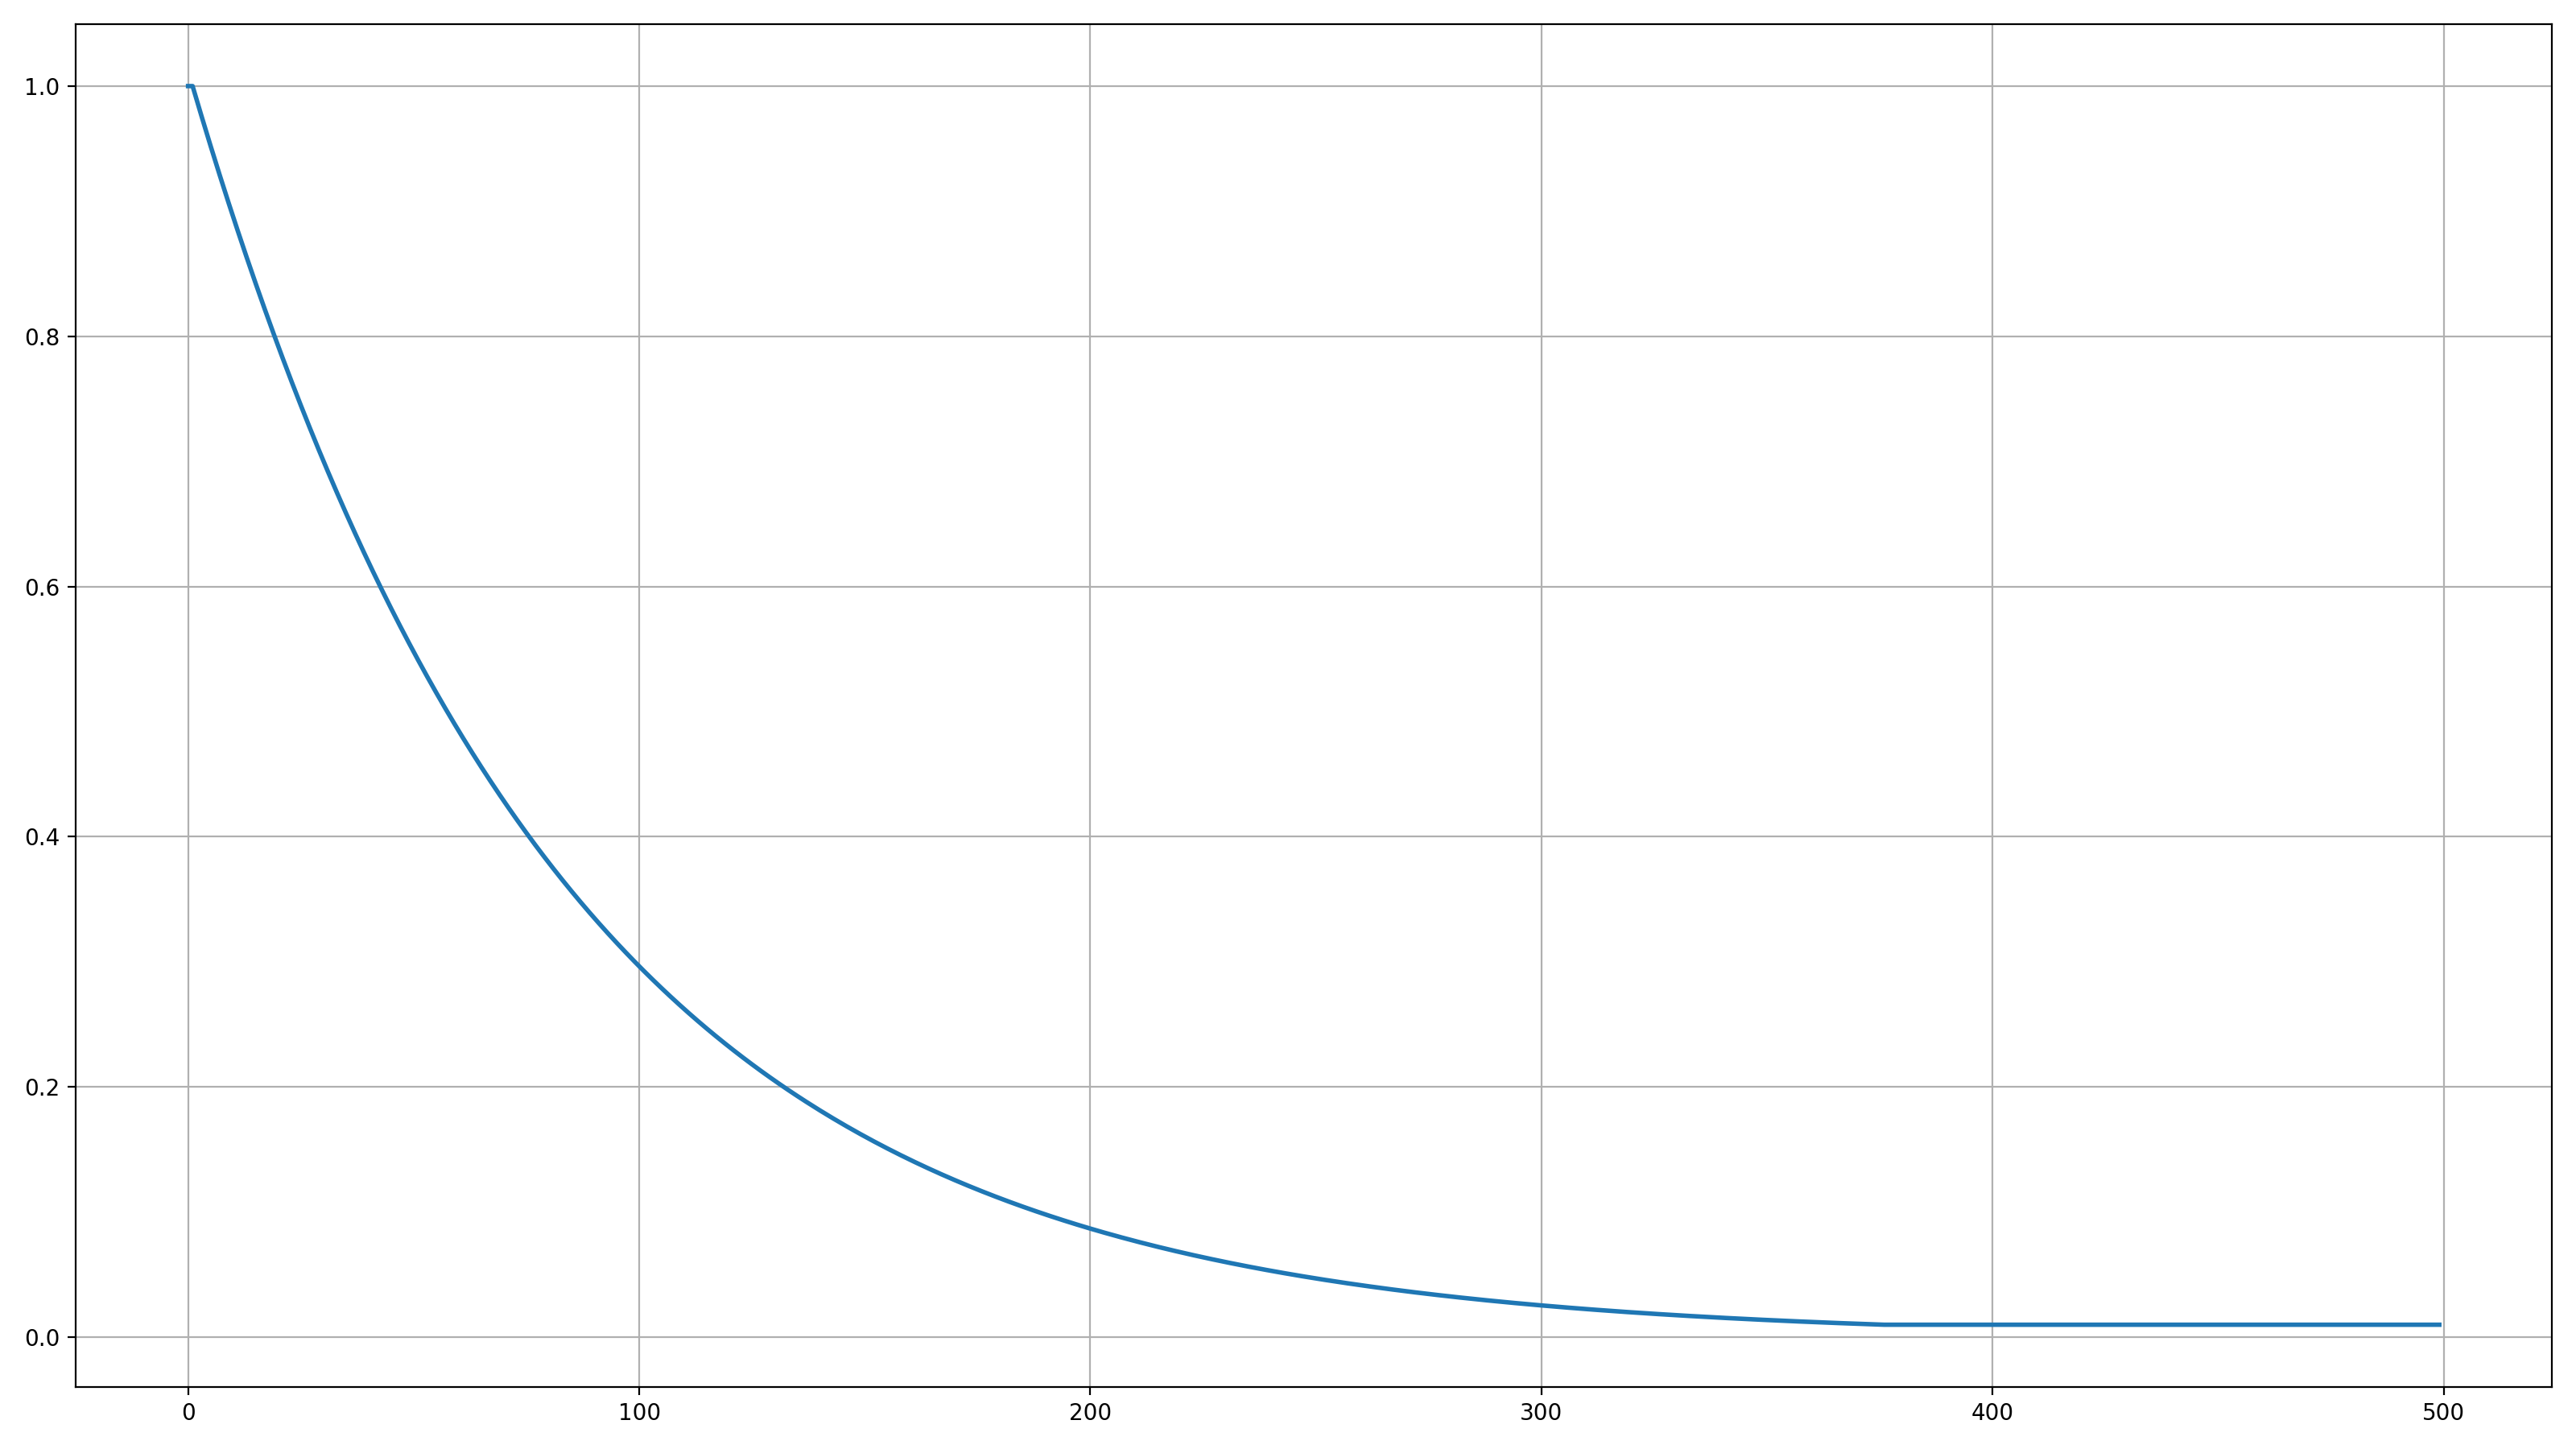
\includegraphics[width=8.5cm]{"../Figures/epsilon_1J_500E_256EL_11RES.png"} \\
	\caption{Epsilon graph over 500 training episodes.}
	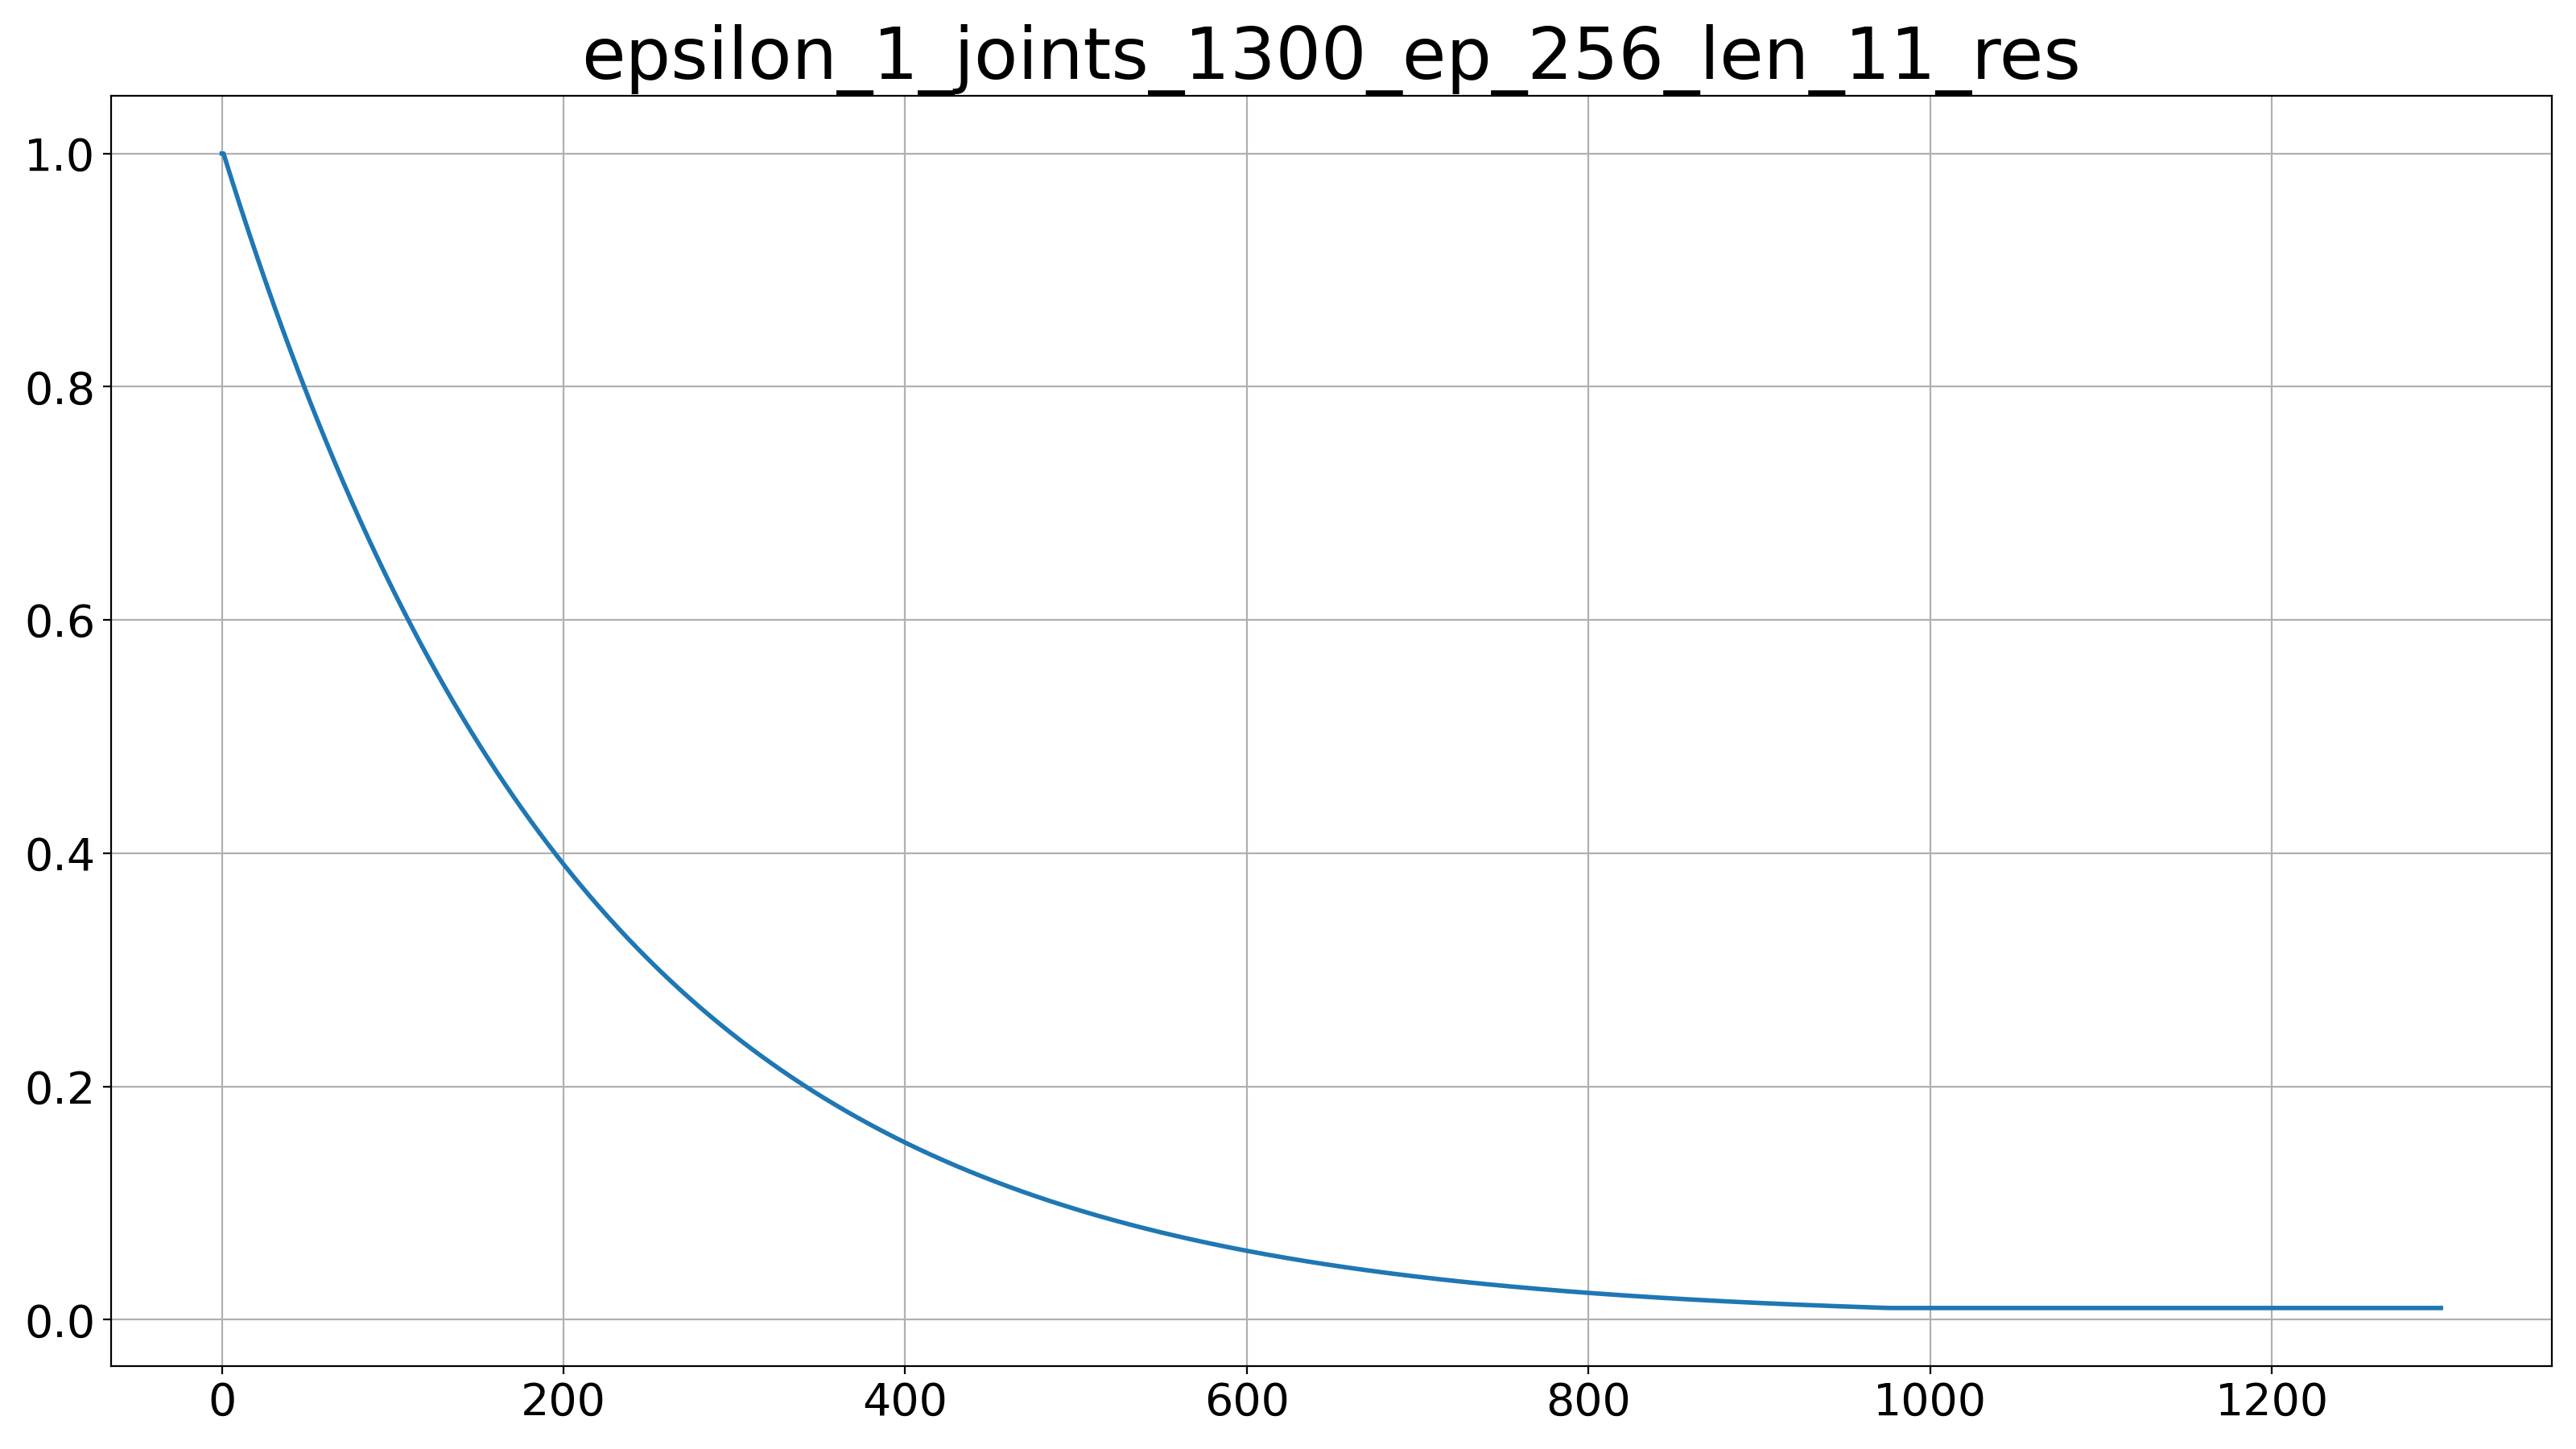
\includegraphics[width=8.5cm]{"../Figures/epsilon_1J_1300E_256EL_11RES.png"}
	\caption{Epsilon graph over 1000 training episodes.}
\end{figure}

\subsection{Actor Network Training}
To run the training the user is required to provide two mandatory values: the
number of episodes and their length, defined as number of steps.
These two parameters define, respectively, the number of the random starting
positions from which the robot will start the training and the length of the
search executed for each episode. At each step, the current state of the
pendulum, \(x_{i}\), is processed by the policy, which produce the control
\(u_{i}\) for this step. The control is applied on the pendulum, producing the
next state \(x_{i+1}\) and the cost \(c_{i}\) of the pair
\((x_{i},u_{i})\). This data are integrated as the transition \(t_{i}=(x_{i},
u_{i}, c_{i}, x_{i+1})\) and added into the experience replay buffer. Once
every \(k_{1}\) steps we proceed to perform a gradient descent execution,
updating the current \(Q\)-network's parameters by sampling a mini-batch of
random transitions from the experience replay buffer and back-propagating the
loss described previously using Adam as optimizer. After gradient descent once
every \(k_{2}\) steps we update the \(Q\)-target network's parameters to match
the current \(Q\) network ones.

\section{Actor Network Testing}
The testing of the actor network was carried out first, varying the starting
position of the robot randomly and secondly making it start from the lowest
position to ensure the goodness of the results.
For each configuration three episodes were run and the sum of costs gathered
during their total length is used as the evaluation measure.
The testing phase works by gathering the robot state, querying the policy
for the next action, apply it and take the cost from the environment for all
the length of the episode.

\section{Experiments}
% 1 joint, 2 joints, N-joints
% Training time
% Changing resolution of the controls
The system has been tested over different configurations of the robot,
specifically with 1 and 2 joints, 11 and 17 control resolution steps and
different numbers of training episodes.
The evaluation metrics used are the loss of the training, the training
cost-to-go at the end of each training episodes and the cumulative cost in the
testing phase.

\section{Results}
\subsection{1 joint}
Following are shown the results in case the robot has 1 joint.

\begin{figure}[H]
	\centering
	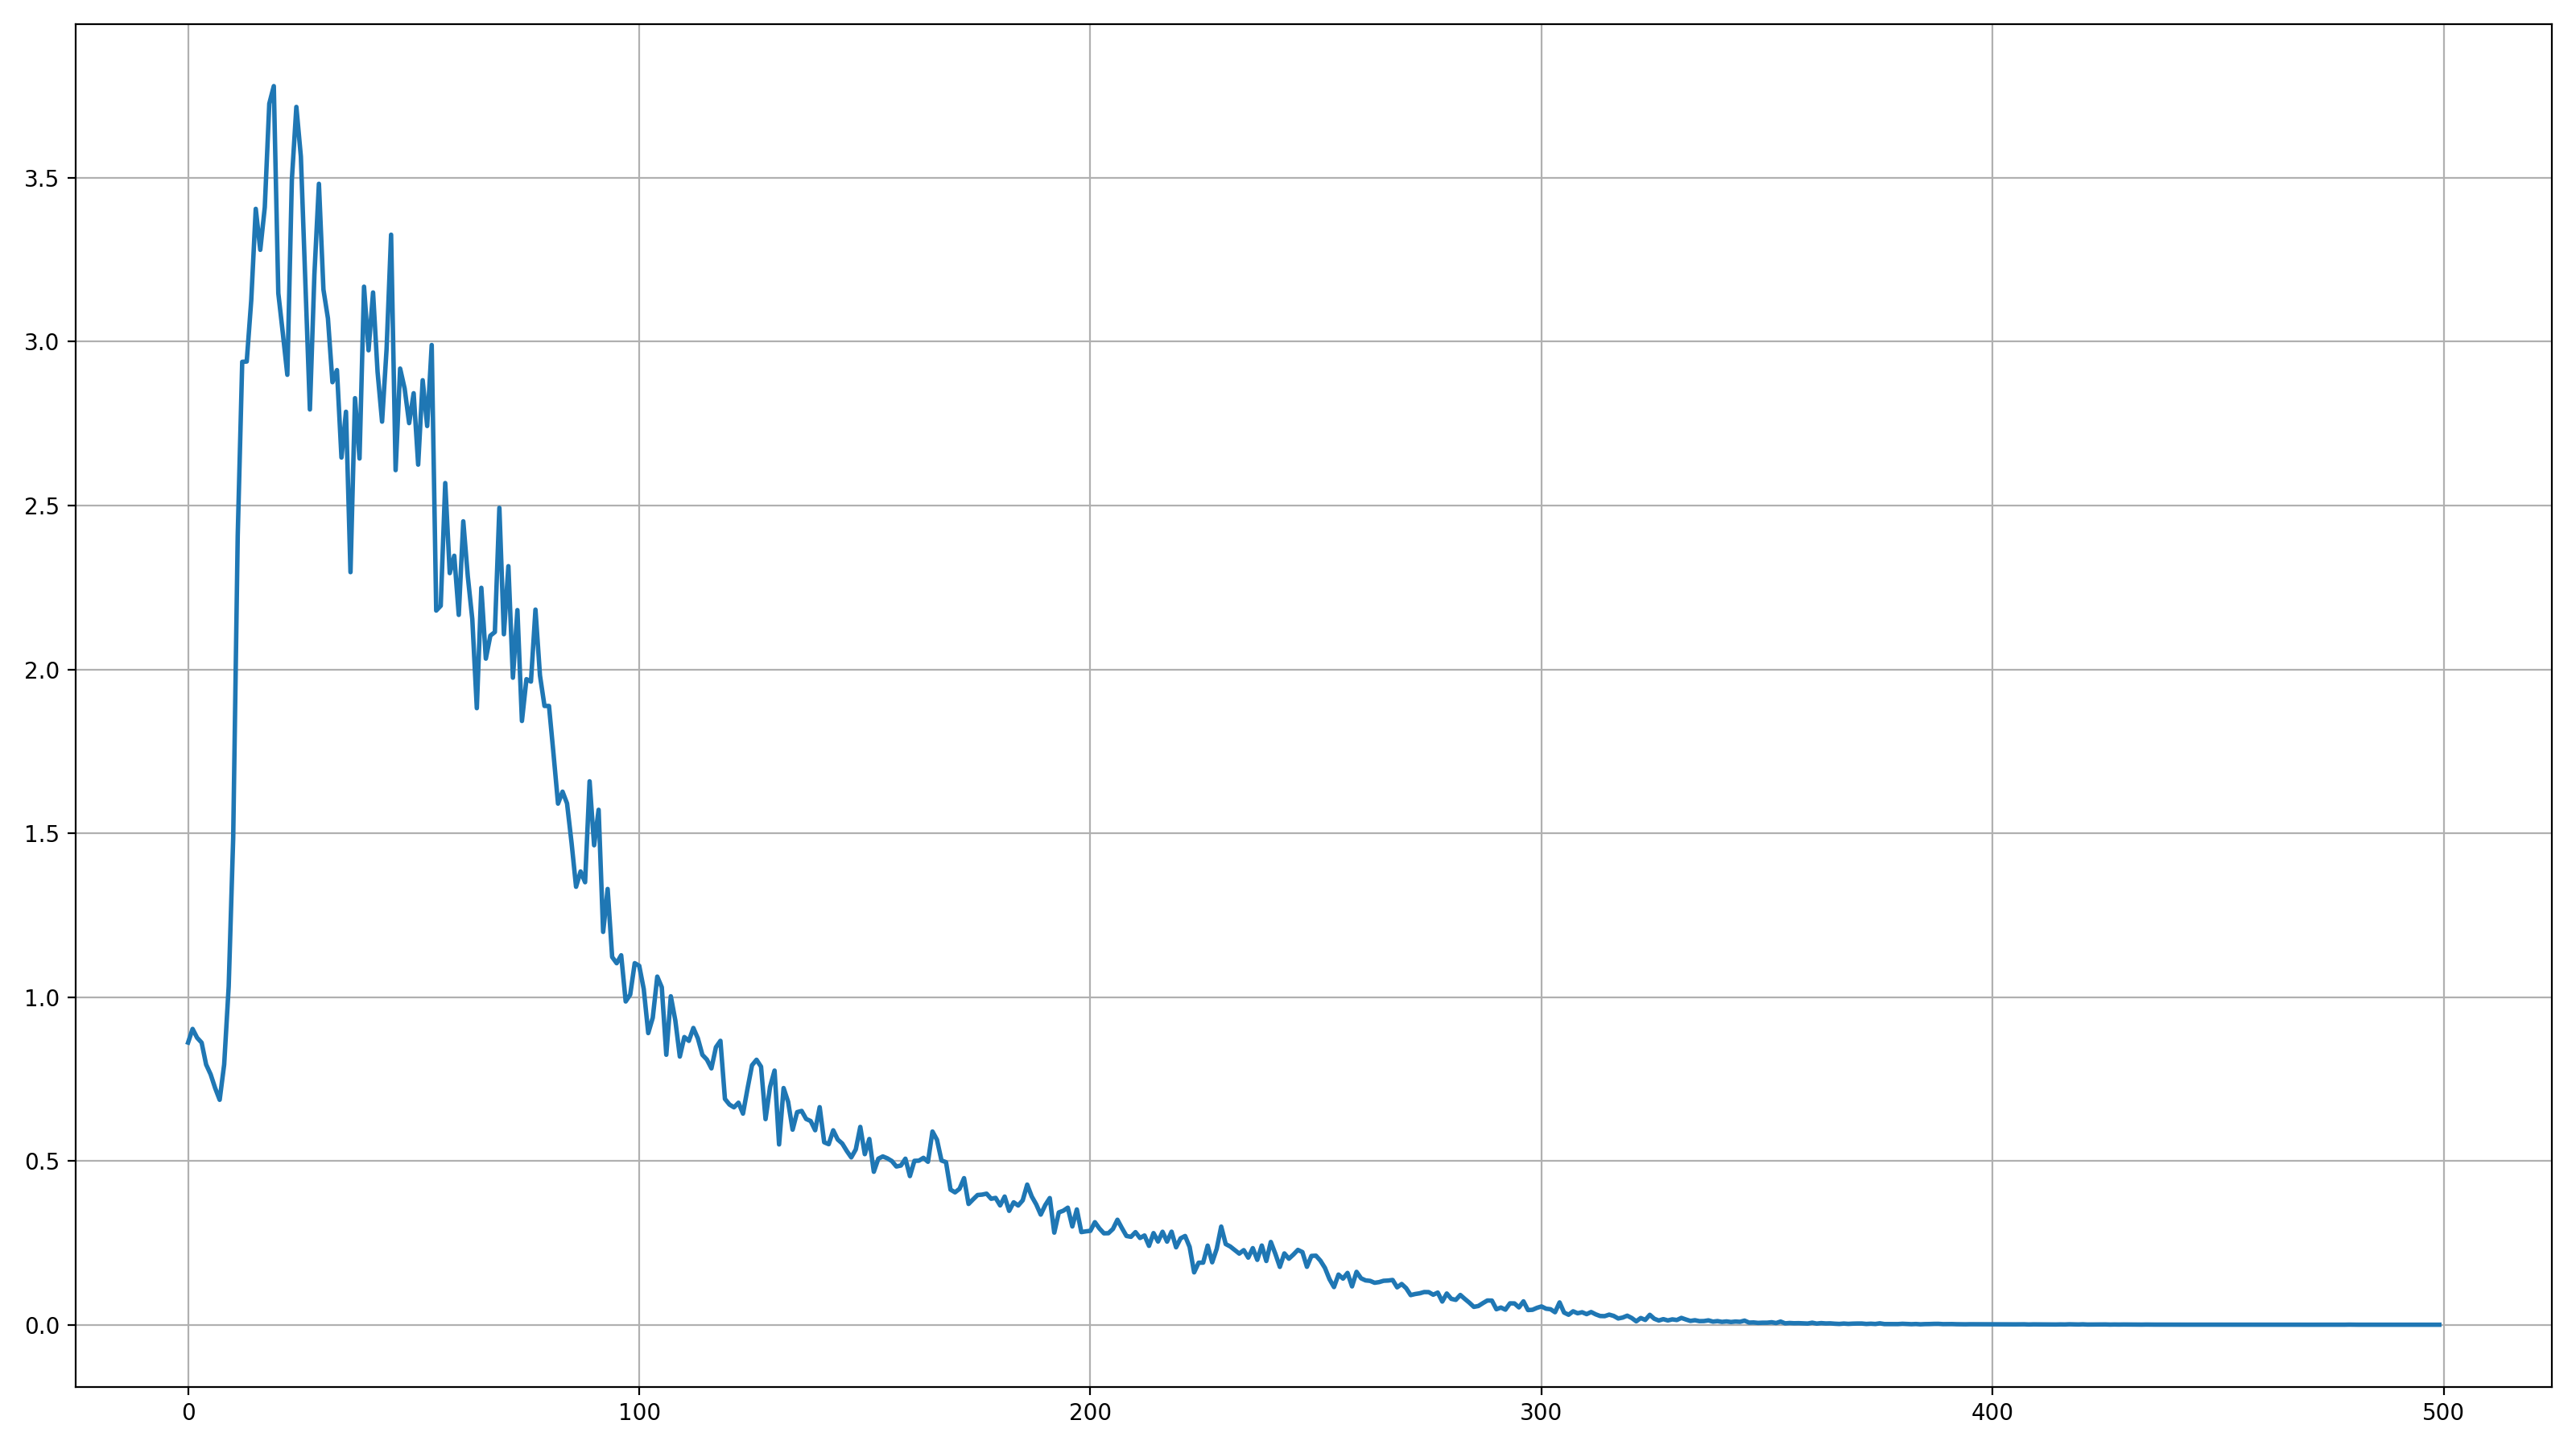
\includegraphics[width=8.5cm]{"../Figures/training_loss_1J_500E_256EL_11RES.png"}
	\caption{Training loss over 500 episodes lasted 256 iterations having 1
			 joint and 11 resolution steps.}
	\label{fig:TrainLoss_1_500_11}
\end{figure}

\begin{figure}[H]
	\centering
	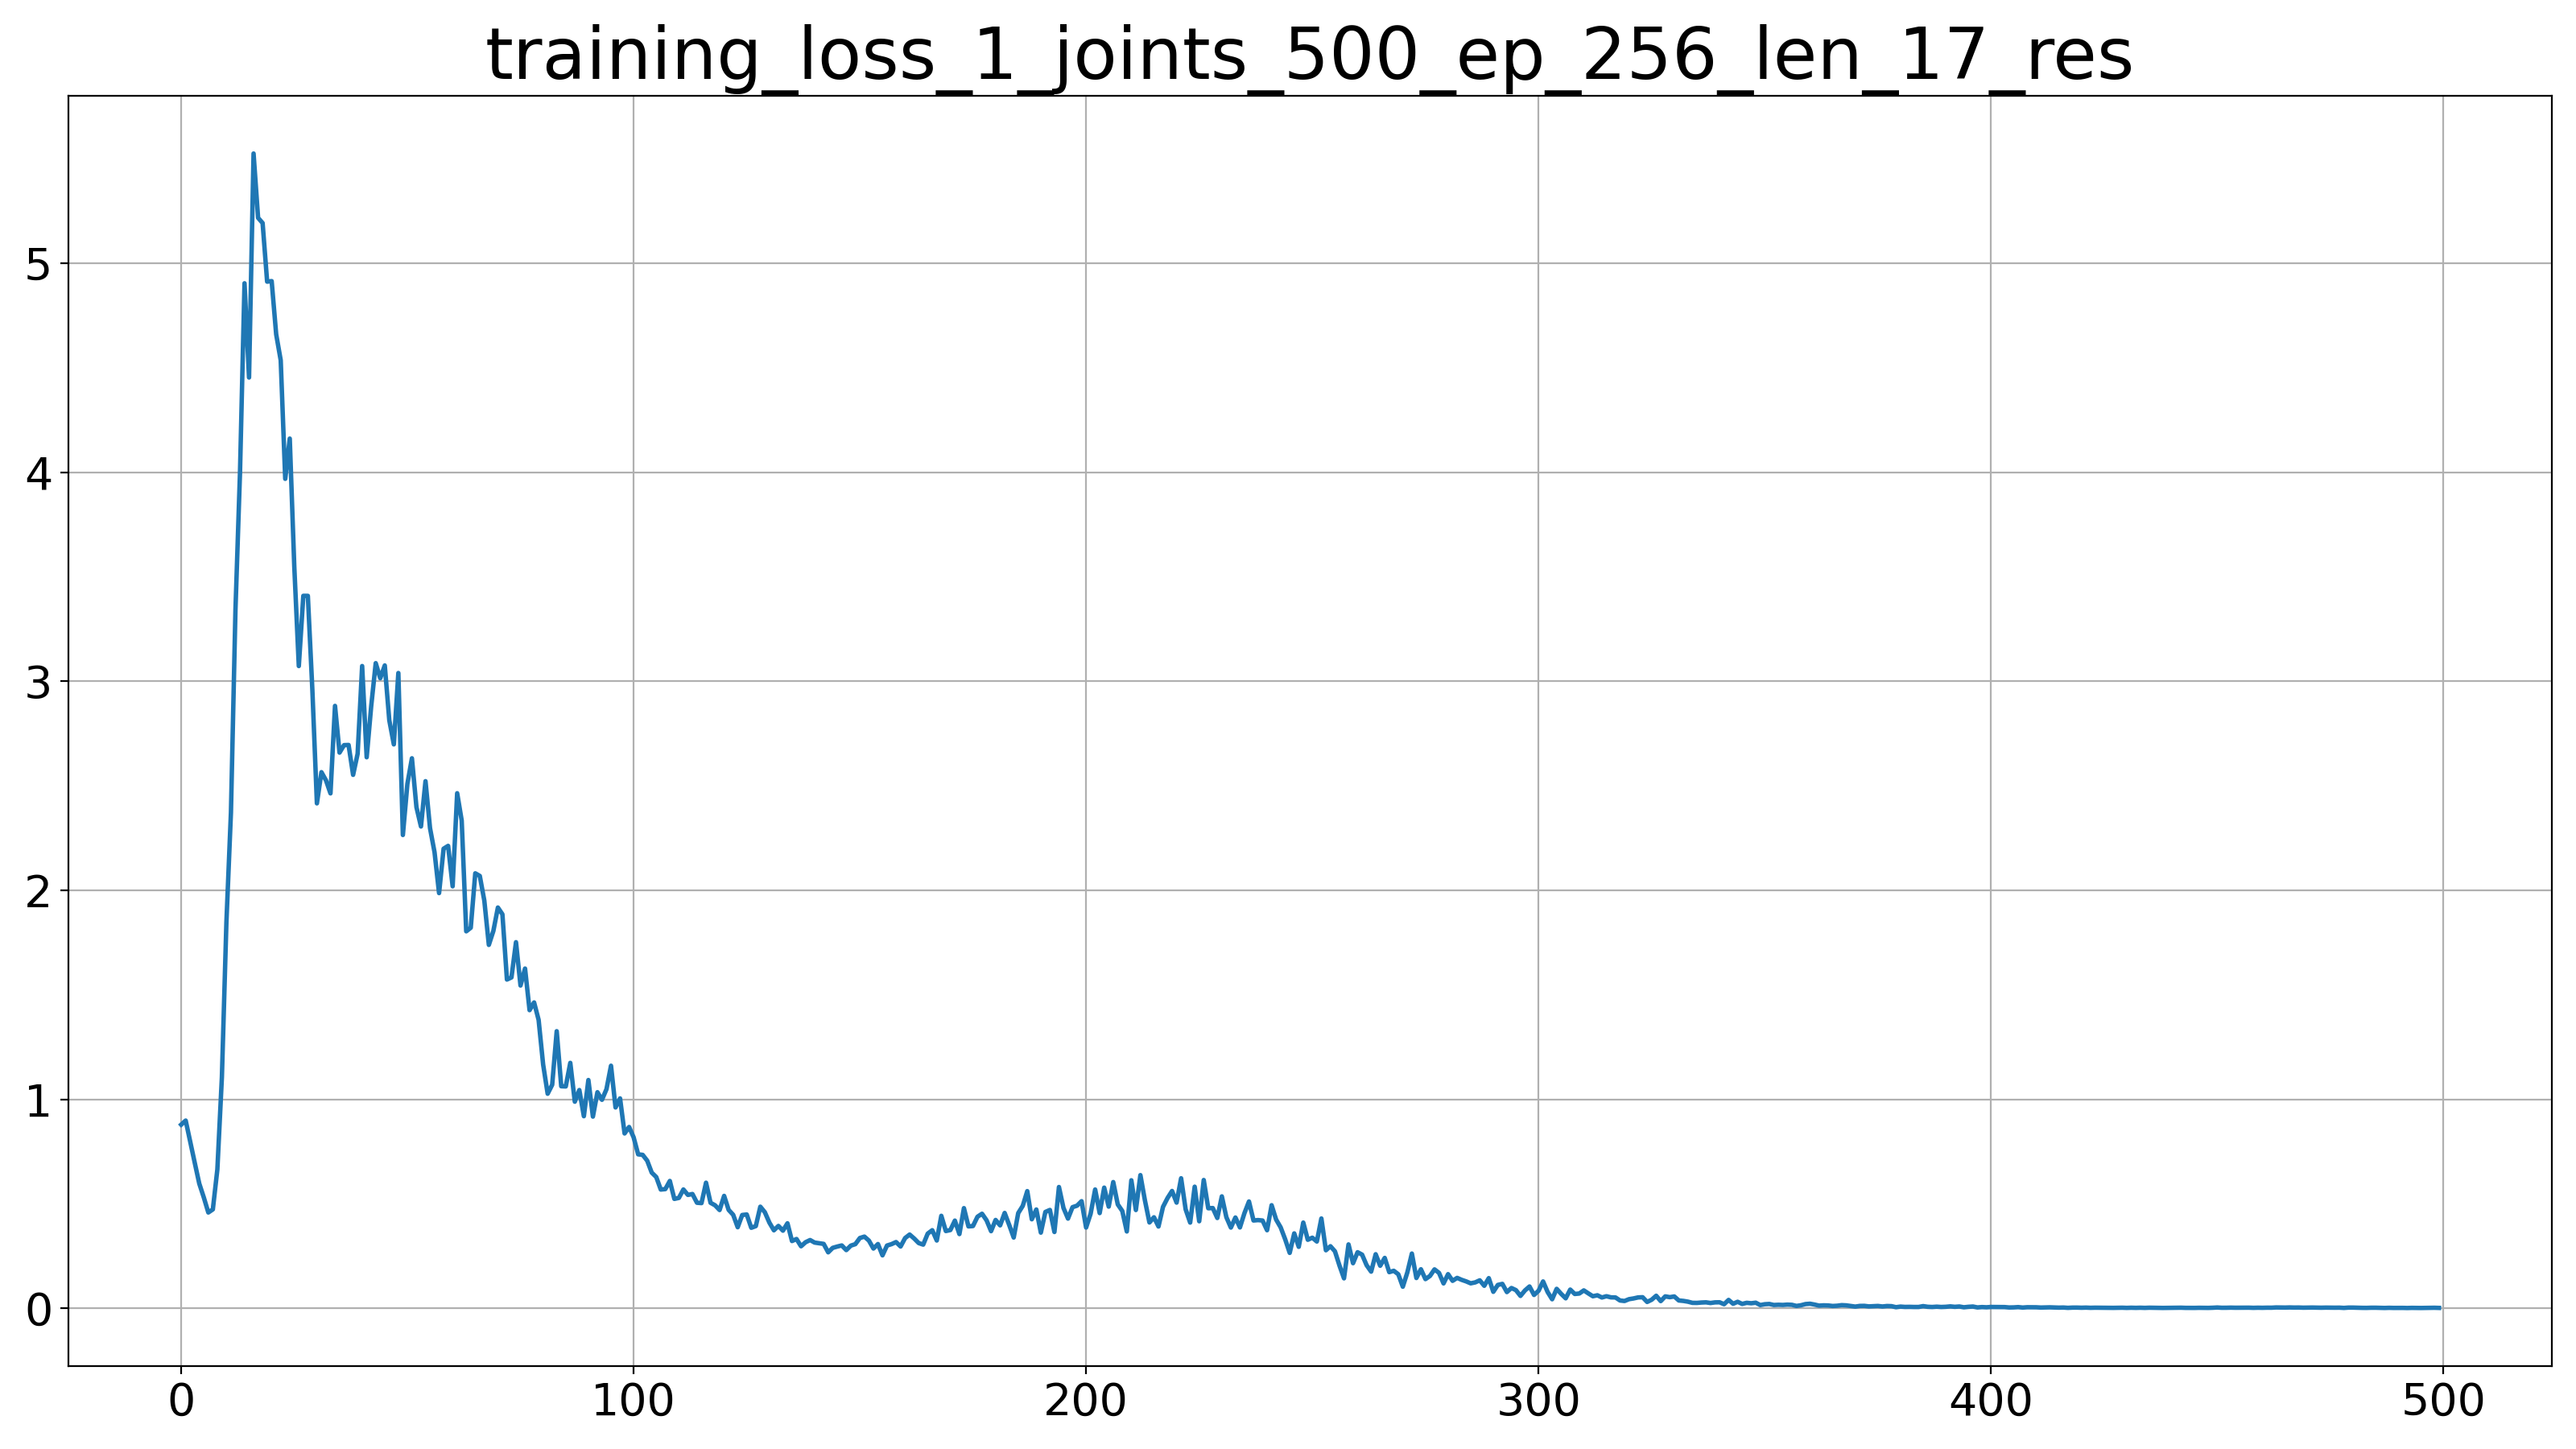
\includegraphics[width=8.5cm]{"../Figures/training_loss_1J_500E_256EL_17RES.png"}
	\caption{Training loss over 500 episodes lasted 256 iterations having 1
			 joint and 17 resolution steps.}
	\label{fig:TrainLoss_1_500_17}
\end{figure}

\begin{figure}[H]
	\centering
	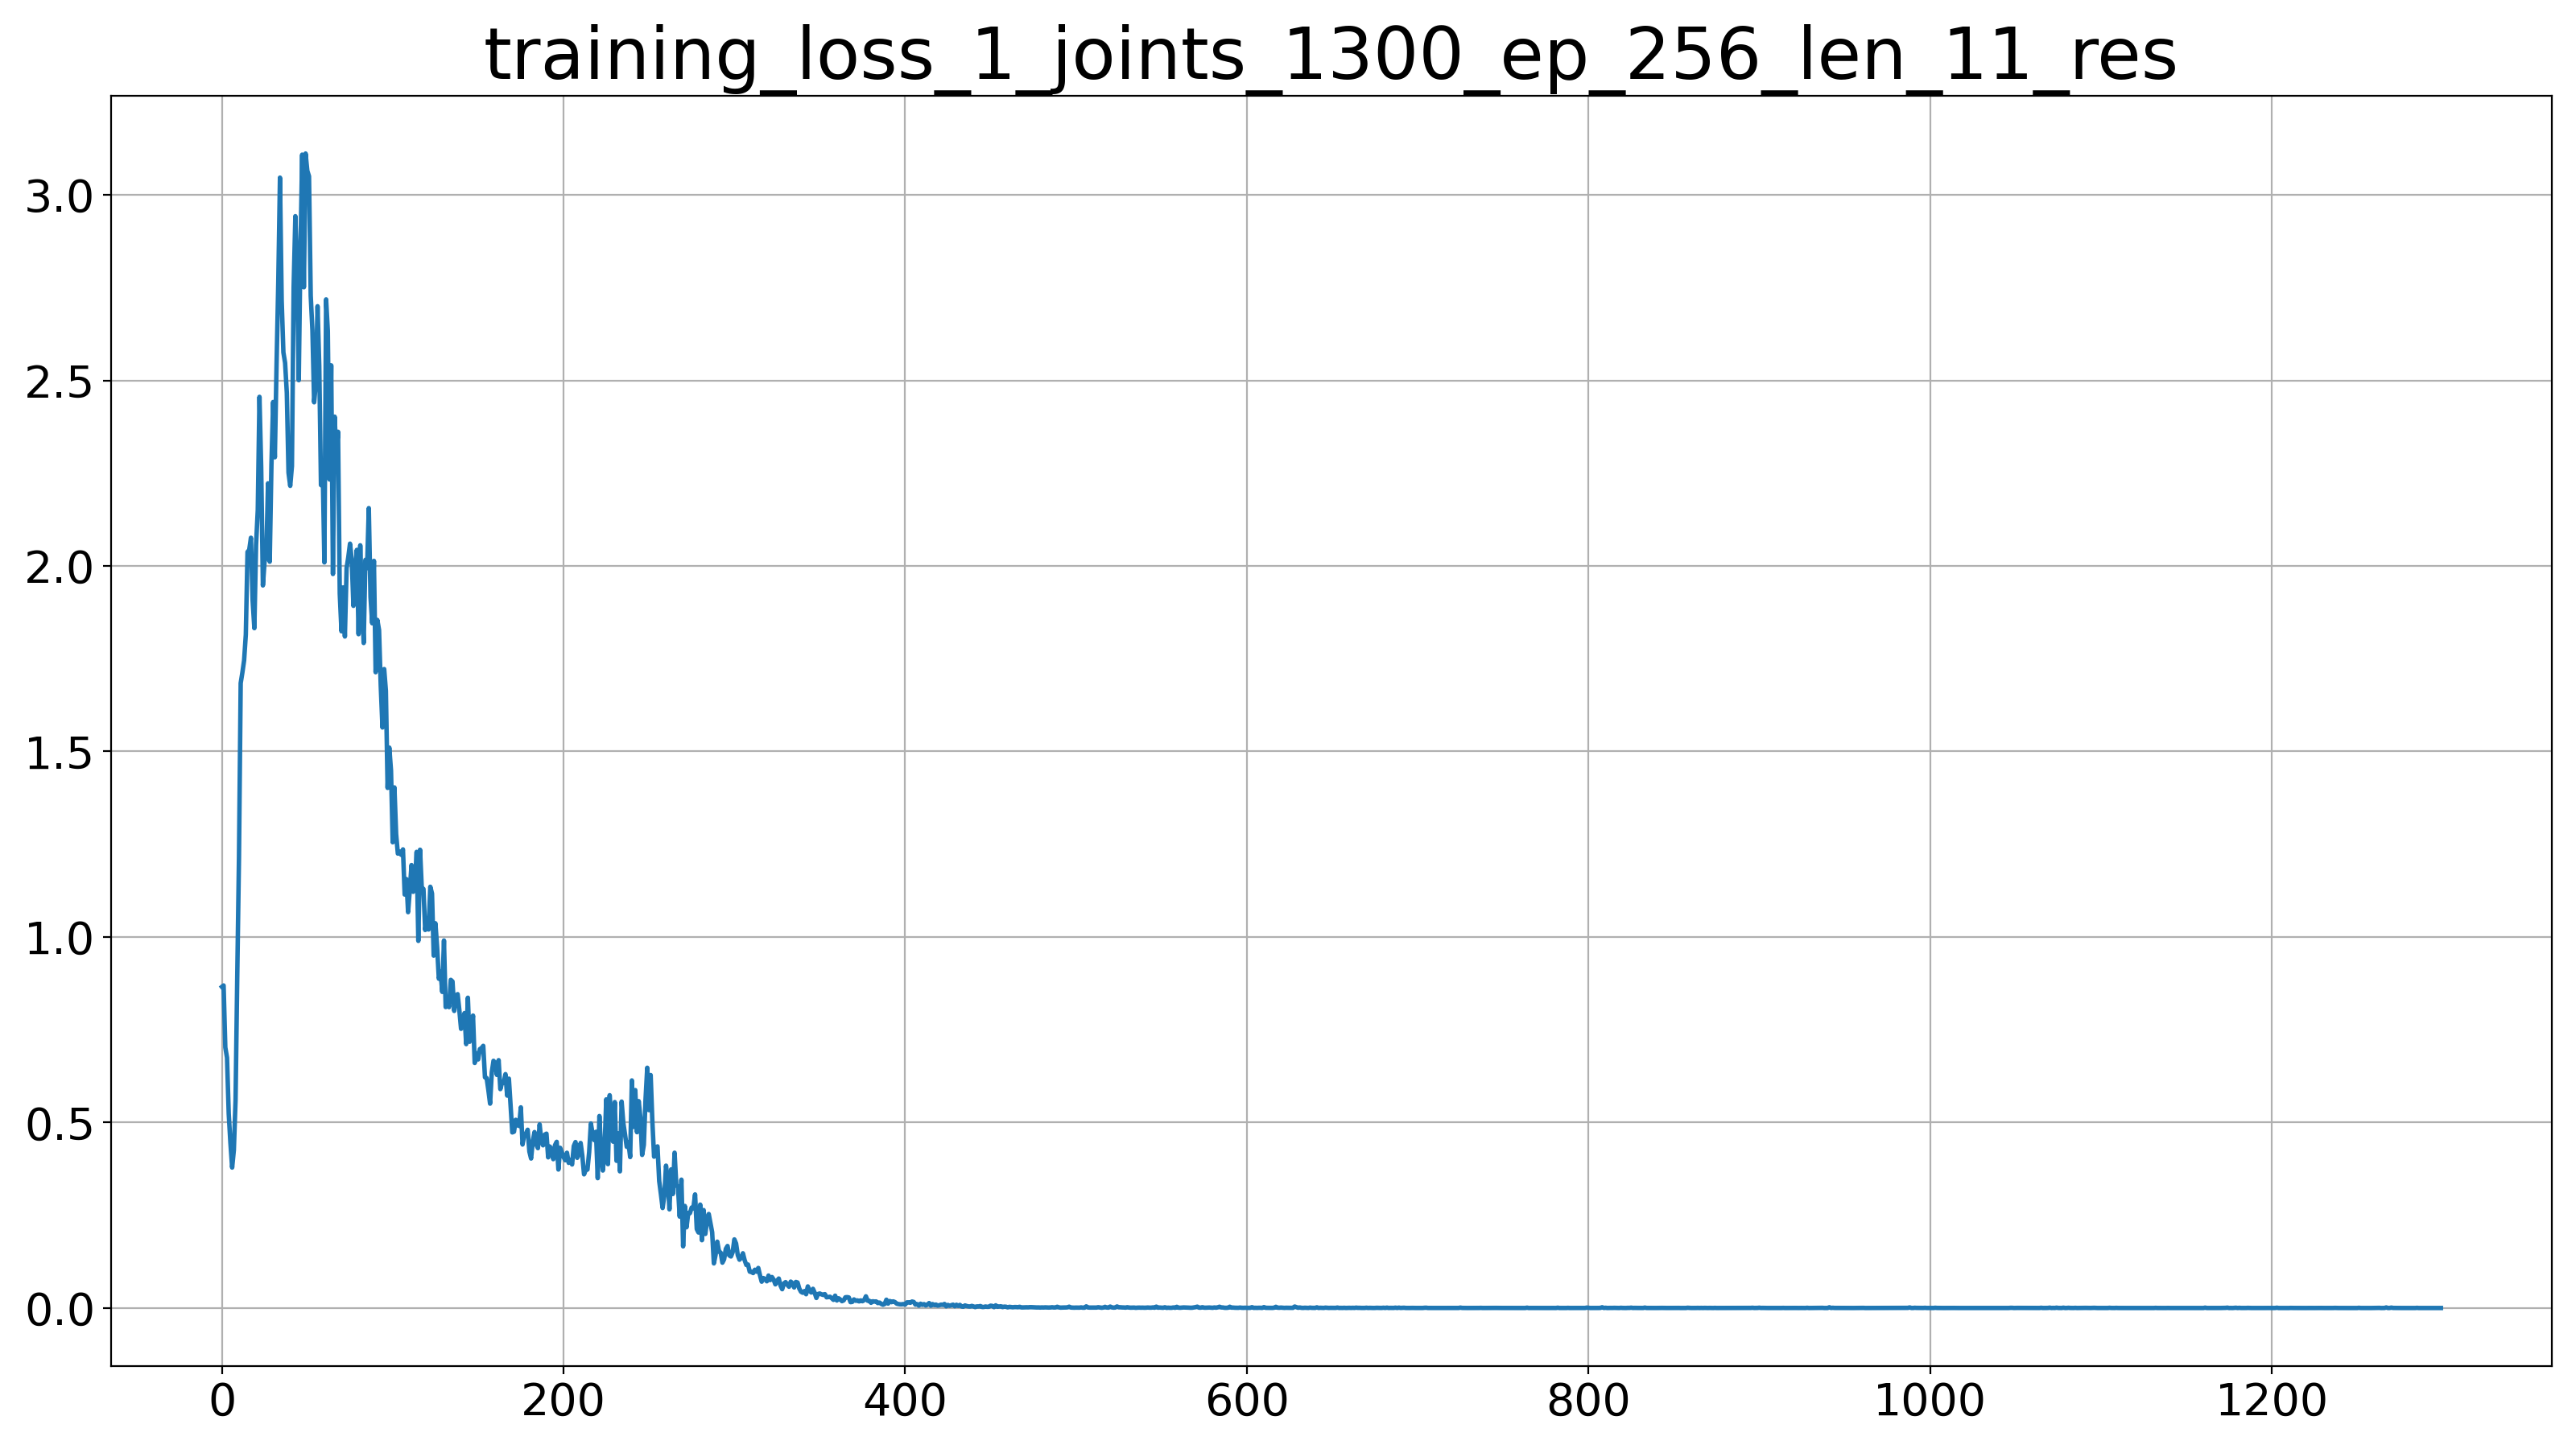
\includegraphics[width=8.5cm]{"../Figures/training_loss_1J_1300E_256EL_11RES.png"}
	\caption{Training loss over 1300 episodes lasted 256 iterations having 1
			 joint and 11 resolution steps.}
	\label{fig:TrainLoss_1_1300_11}
\end{figure}

\begin{figure}[H]
	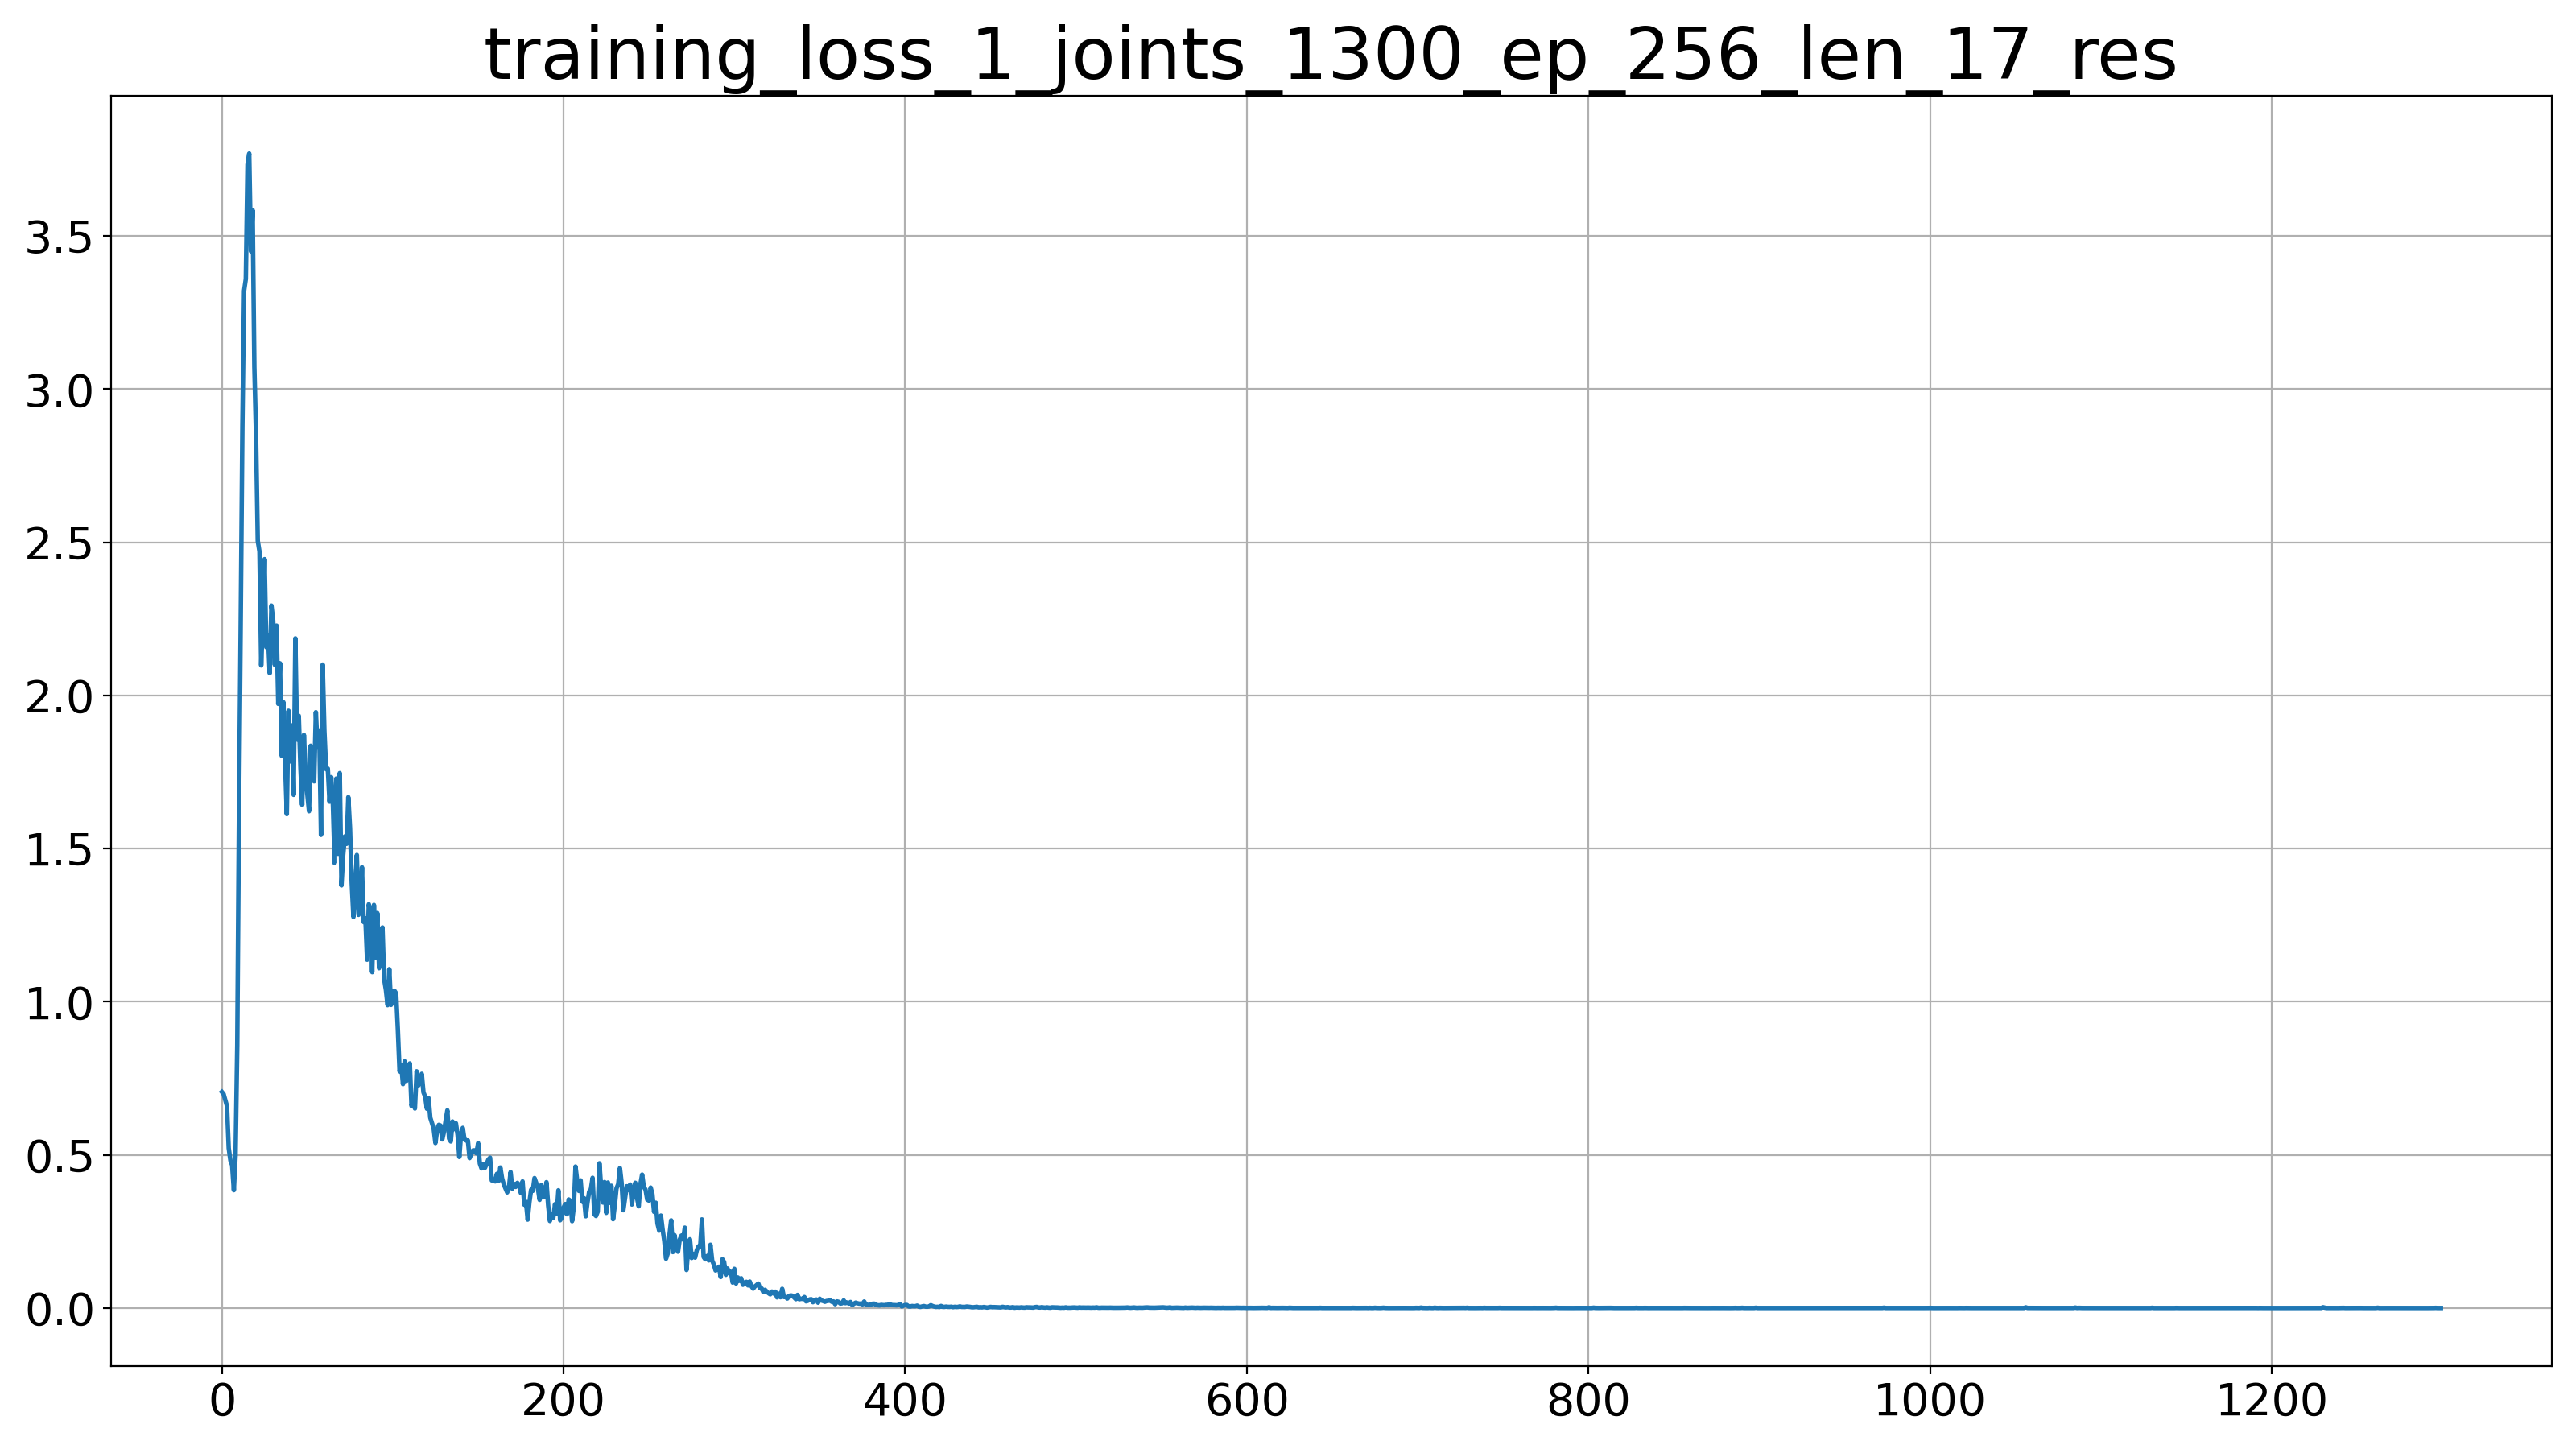
\includegraphics[width=8.5cm]{"../Figures/training_loss_1J_1300E_256EL_17RES.png"}
	\caption{Training loss over 1300 episodes lasted 256 iterations having 1
			 joint and 17 resolution steps.}
	\label{fig:TrainLoss_1_1300_17}
\end{figure}

% Training_cost_to_go
Together with the training loss, it is also important to observe the behaviour
of the episodes cost to go at the end of their length.

\begin{figure}[H]
	\centering
	\includegraphics[width=8.5cm]{"../Figures/Training_costs_1_joints_500_ep_256_len_11_res.png"}
	\caption{Training cost-to-go over 500 episodes lasted 256 iterations having 1
			 joint and 11 resolution steps.}
	\label{fig:Train_cost_to_go_1_500_11}
\end{figure}

\begin{figure}[H]
	\includegraphics[width=8.5cm]{"../Figures/Training_costs_1_joints_500_ep_256_len_17_res.png"}
	\caption{Training cost-to-go over 500 episodes lasted 256 iterations having 1
			 joint and 17 resolution steps.}
	\label{fig:Train_cost_to_go_1_500_17}
\end{figure}

\begin{figure}[H]
	\includegraphics[width=8.5cm]{"../Figures/Training_costs_1_joints_1300_ep_256_len_11_res.png"}
	\caption{Training cost-to-go over 1300 episodes lasted 256 iterations having 1
			 joint and 11 resolution steps.}
	\label{fig:Train_cost_to_go_1_1300_11}
\end{figure}
\begin{figure}[H]
	\includegraphics[width=8.5cm]{"../Figures/Training_costs_1_joints_1300_ep_256_len_17_res.png"}
	\caption{Training cost-to-go over 1300 episodes lasted 256 iterations having 1
			 joint and 17 resolution steps.}
	\label{fig:Train_cost_to_go_1_1300_17}
\end{figure}

As shown in the graphs, the cost keeps decreasing until it reaches convergence
in the latter episodes of the training, as shown in Figures
\ref{fig:Train_cost_to_go_1_500_11} and \ref{fig:Train_cost_to_go_1_500_17}
where it converges at around the $400^{th}$ episode, while using more
training episodes also the convergence point is moved further in time as shown
by Figures \ref{fig:Train_cost_to_go_1_1300_11} and
\ref{fig:Train_cost_to_go_1_1300_17}
where convergence is reached towards the $600^{th}$ episode.

% Test phase
\begin{figure}[H]
	\centering
	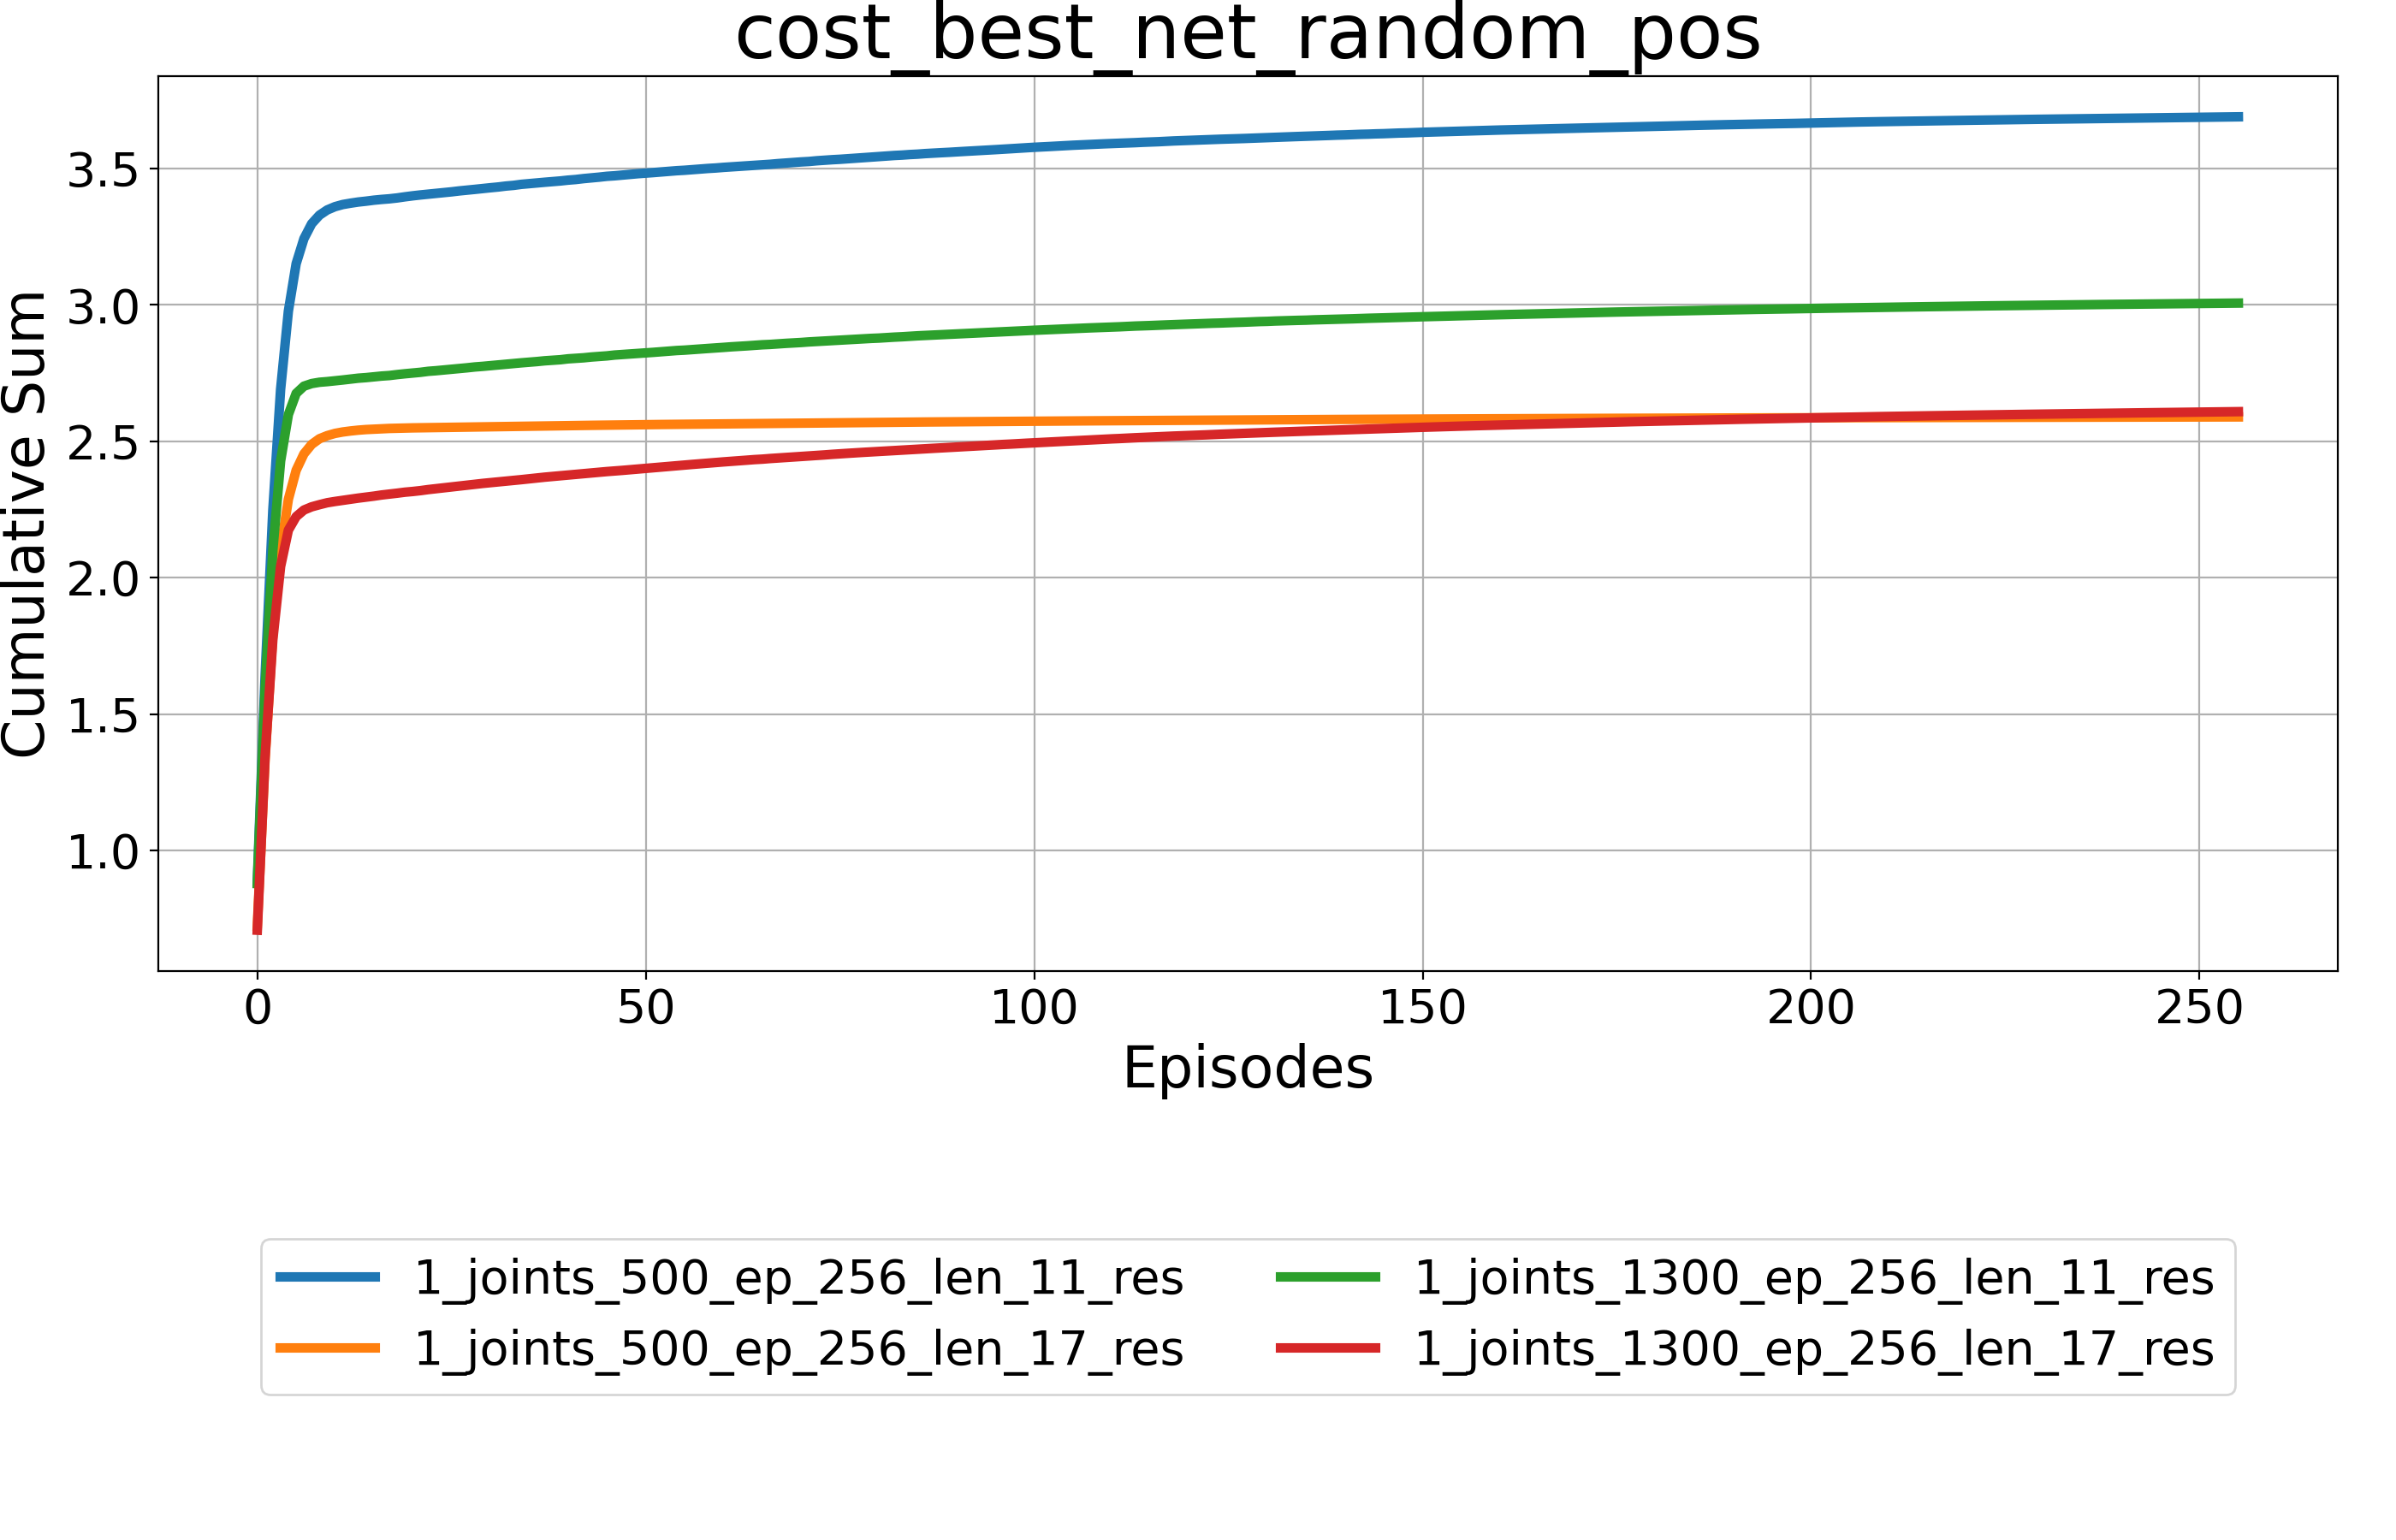
\includegraphics[width=8.5cm]{"../Figures/Summary_cost_best_net_random_pos_1J.png"}
	\caption{Total cost over the test episodes for the robot starting from
			 random positions using the best performing network.}
	\label{fig:Test_1_best_net_random_pos}
\end{figure}


\begin{figure}[H]
	\centering
	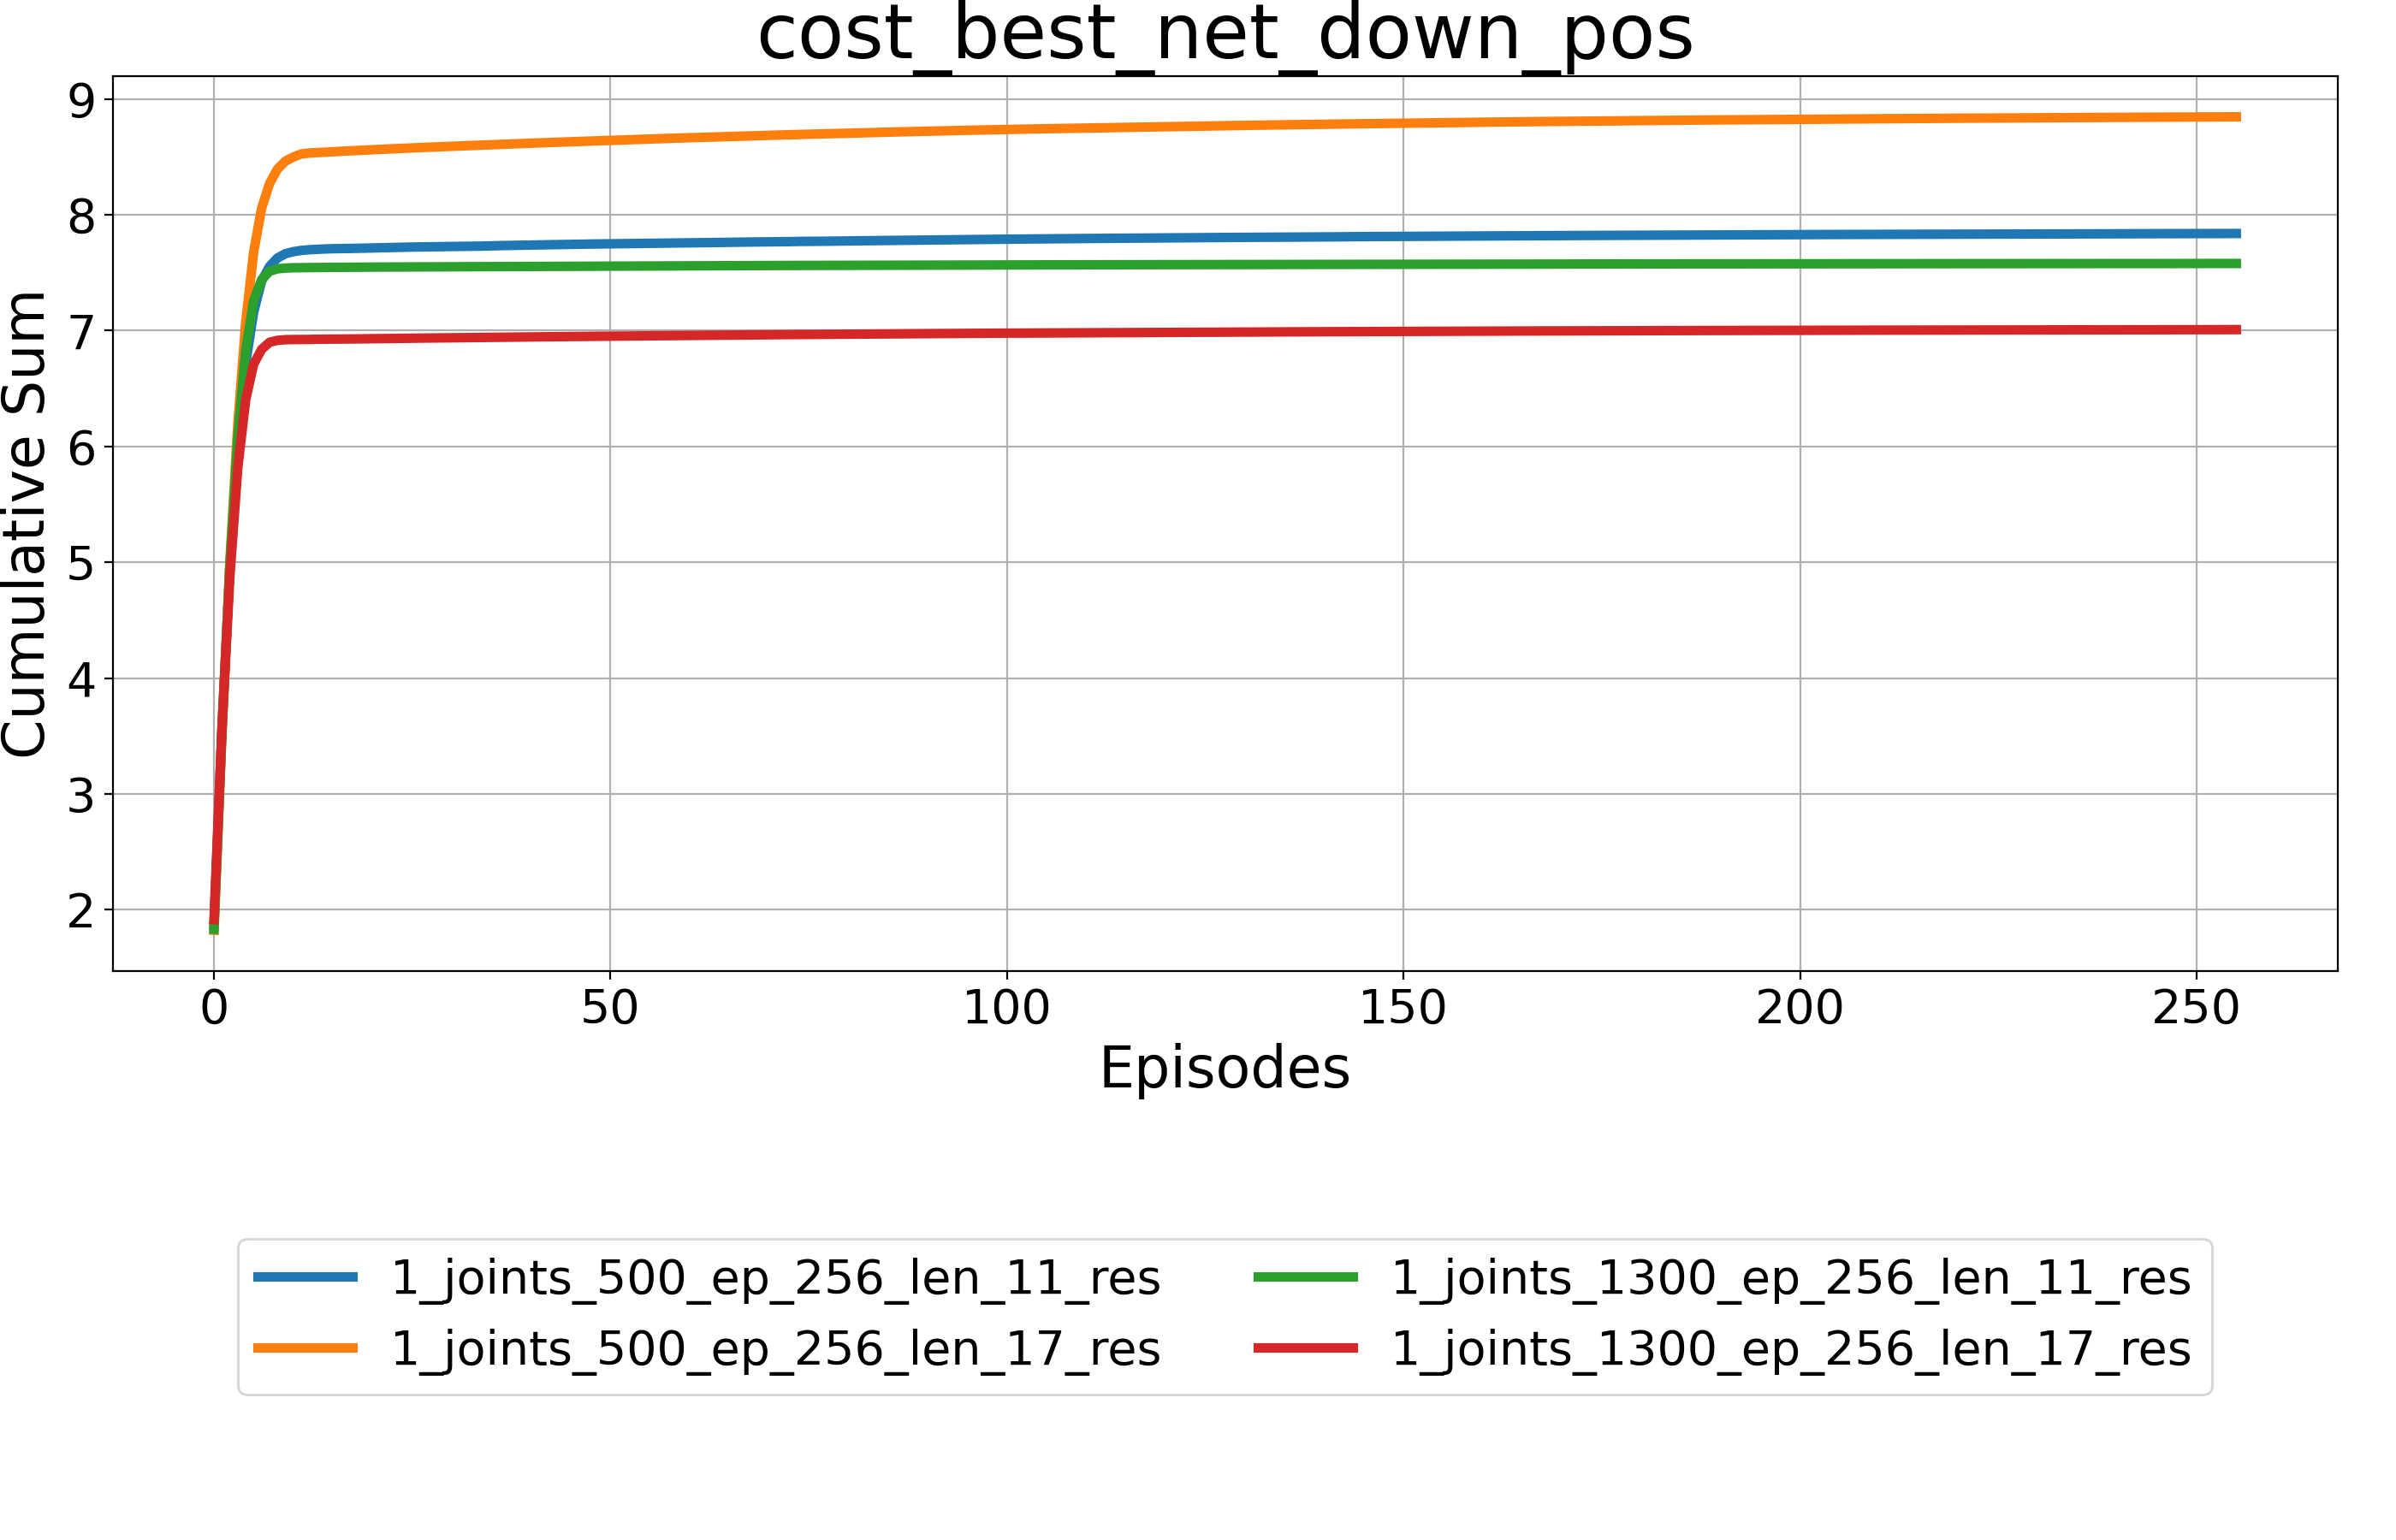
\includegraphics[width=8.5cm]{"../Figures/Summary_cost_best_net_down_pos_1J.png"}
	\caption{Total cost over the test episodes for the robot starting from
			 down positions using the best performing network.}
	\label{fig:Test_1_best_net_down_pos}
\end{figure}

\subsection{2 joints}
Following are shown the results in case the robot has 2 joints.

\begin{figure}[H]
	\centering
	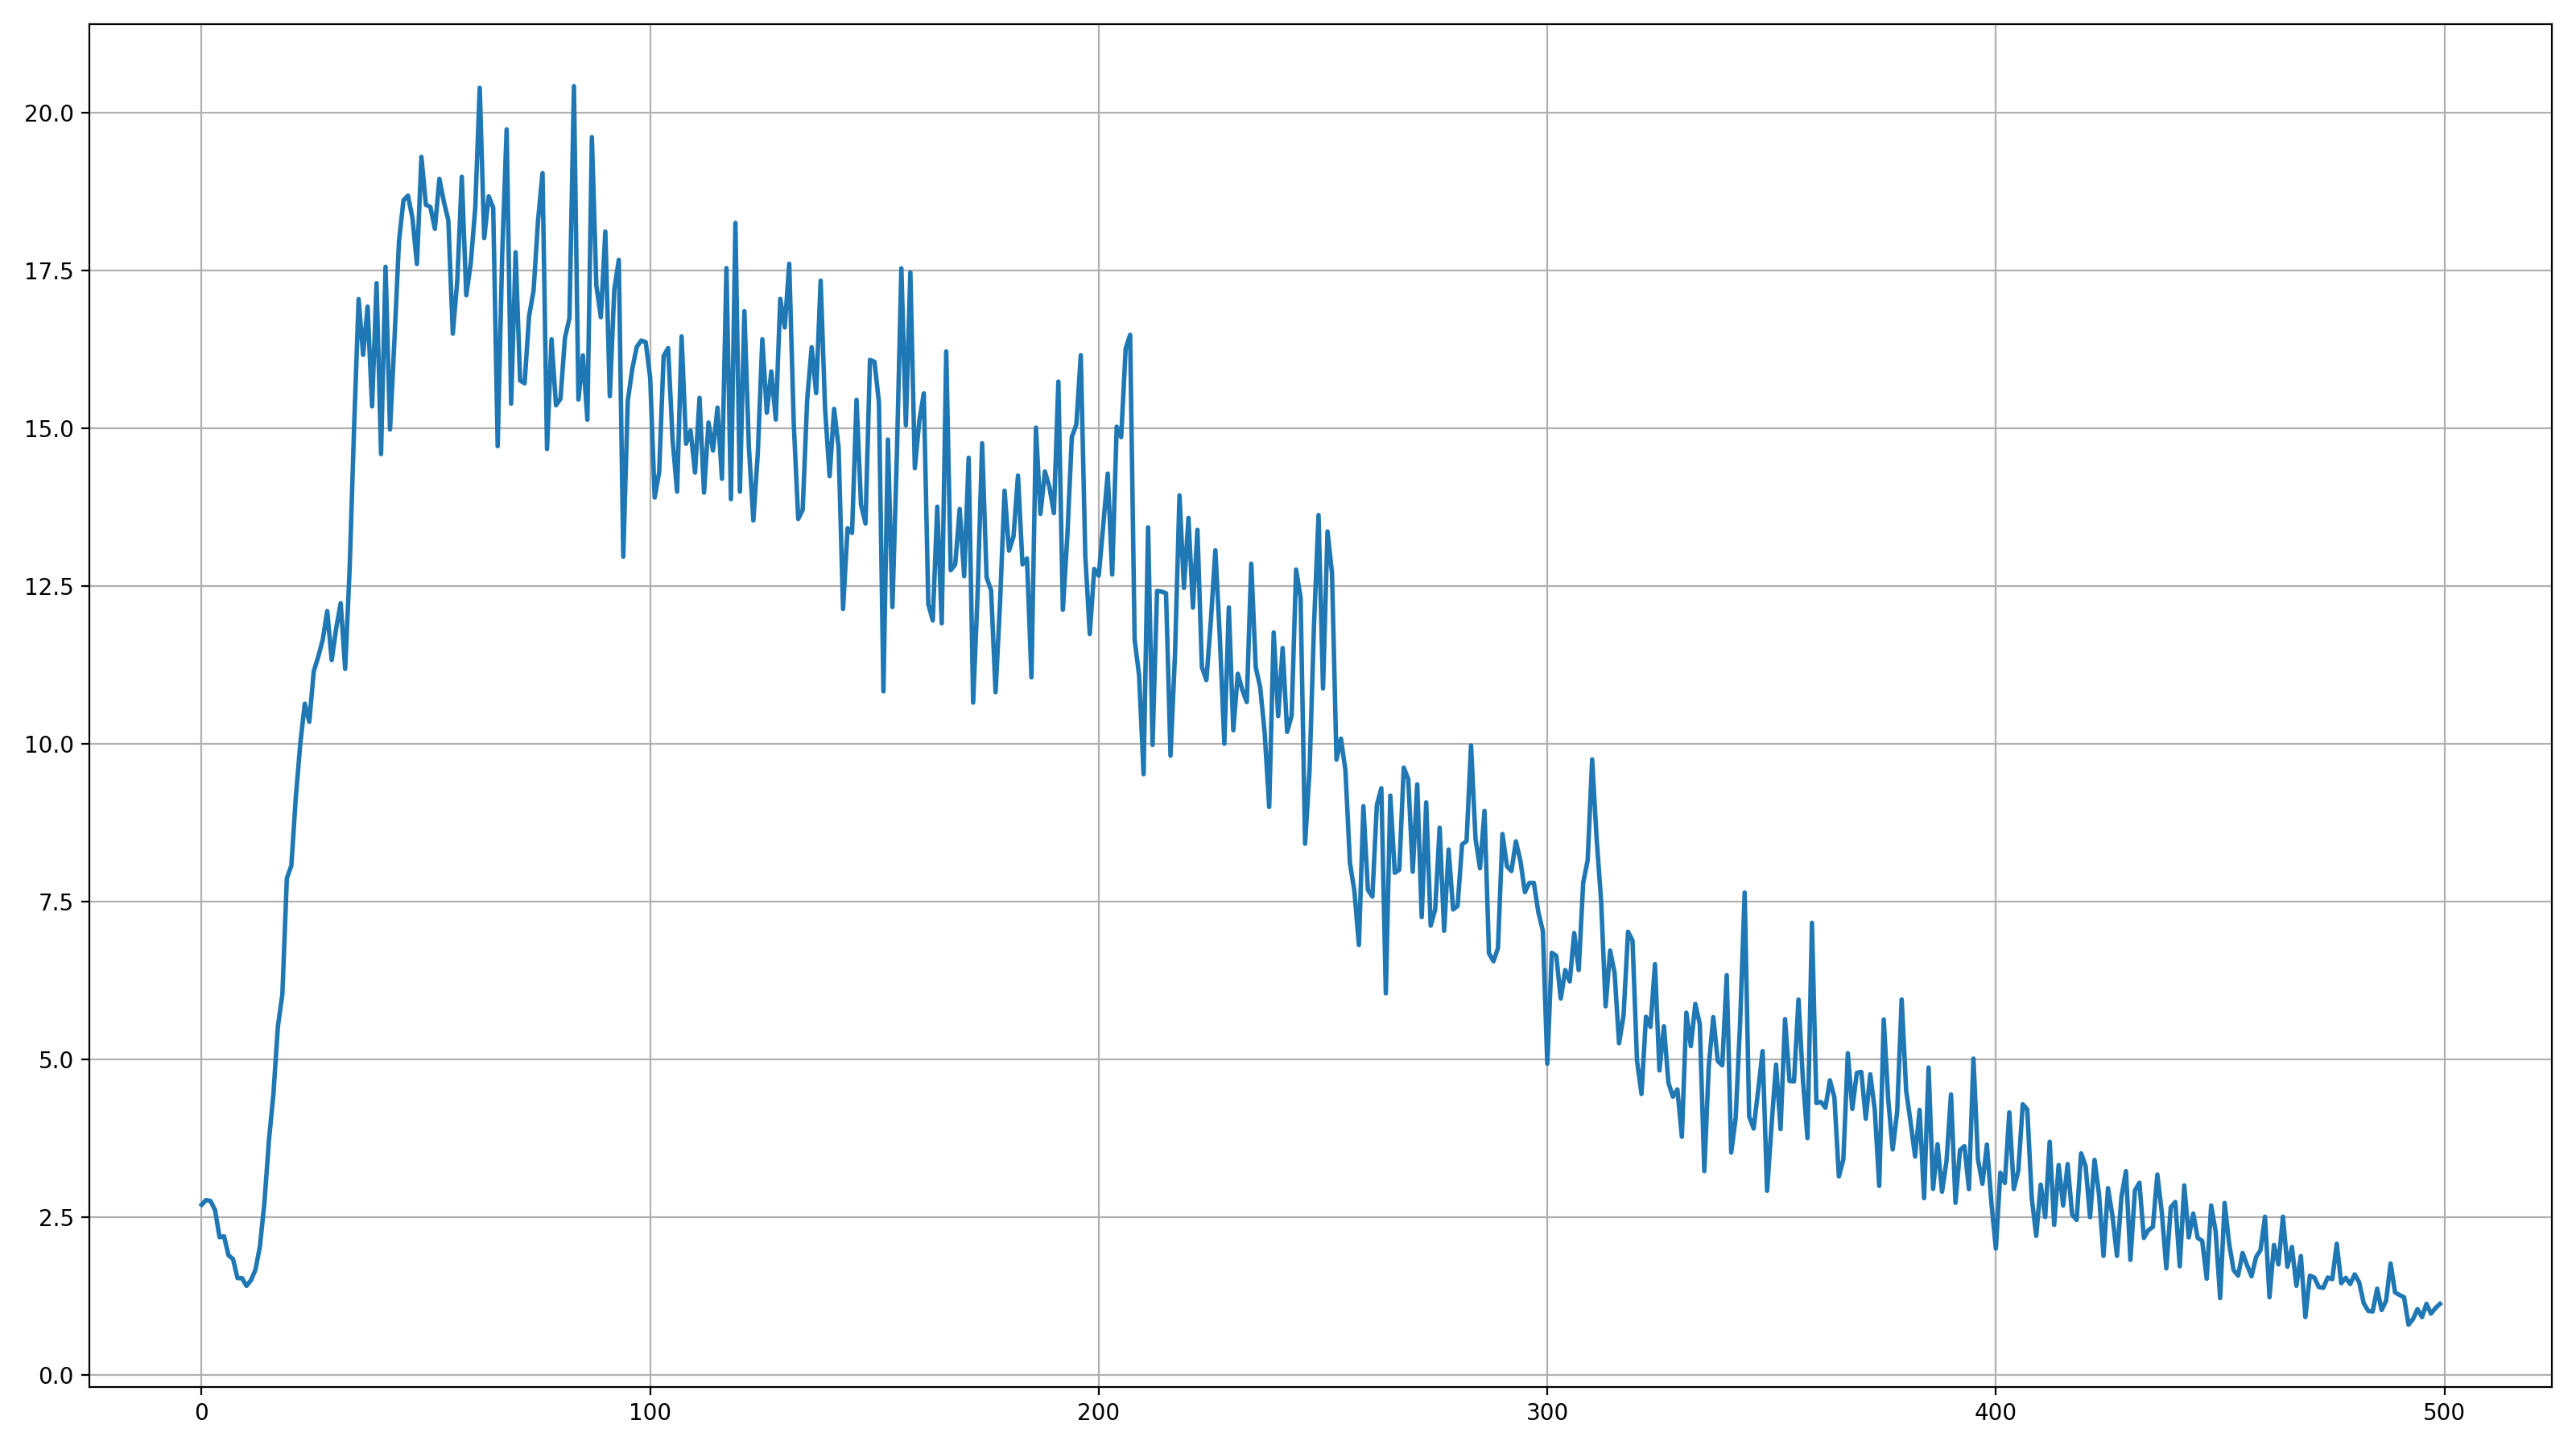
\includegraphics[width=8.5cm]{"../Figures/training_loss_2J_500E_256EL_11RES.png"}
	\caption{Training loss over 500 episodes lasted 256 iterations having 2
			 joint and 11 resolution steps.}
	\label{fig:TrainLoss_2_500_11}
\end{figure}

\begin{figure}[H]
	\centering
	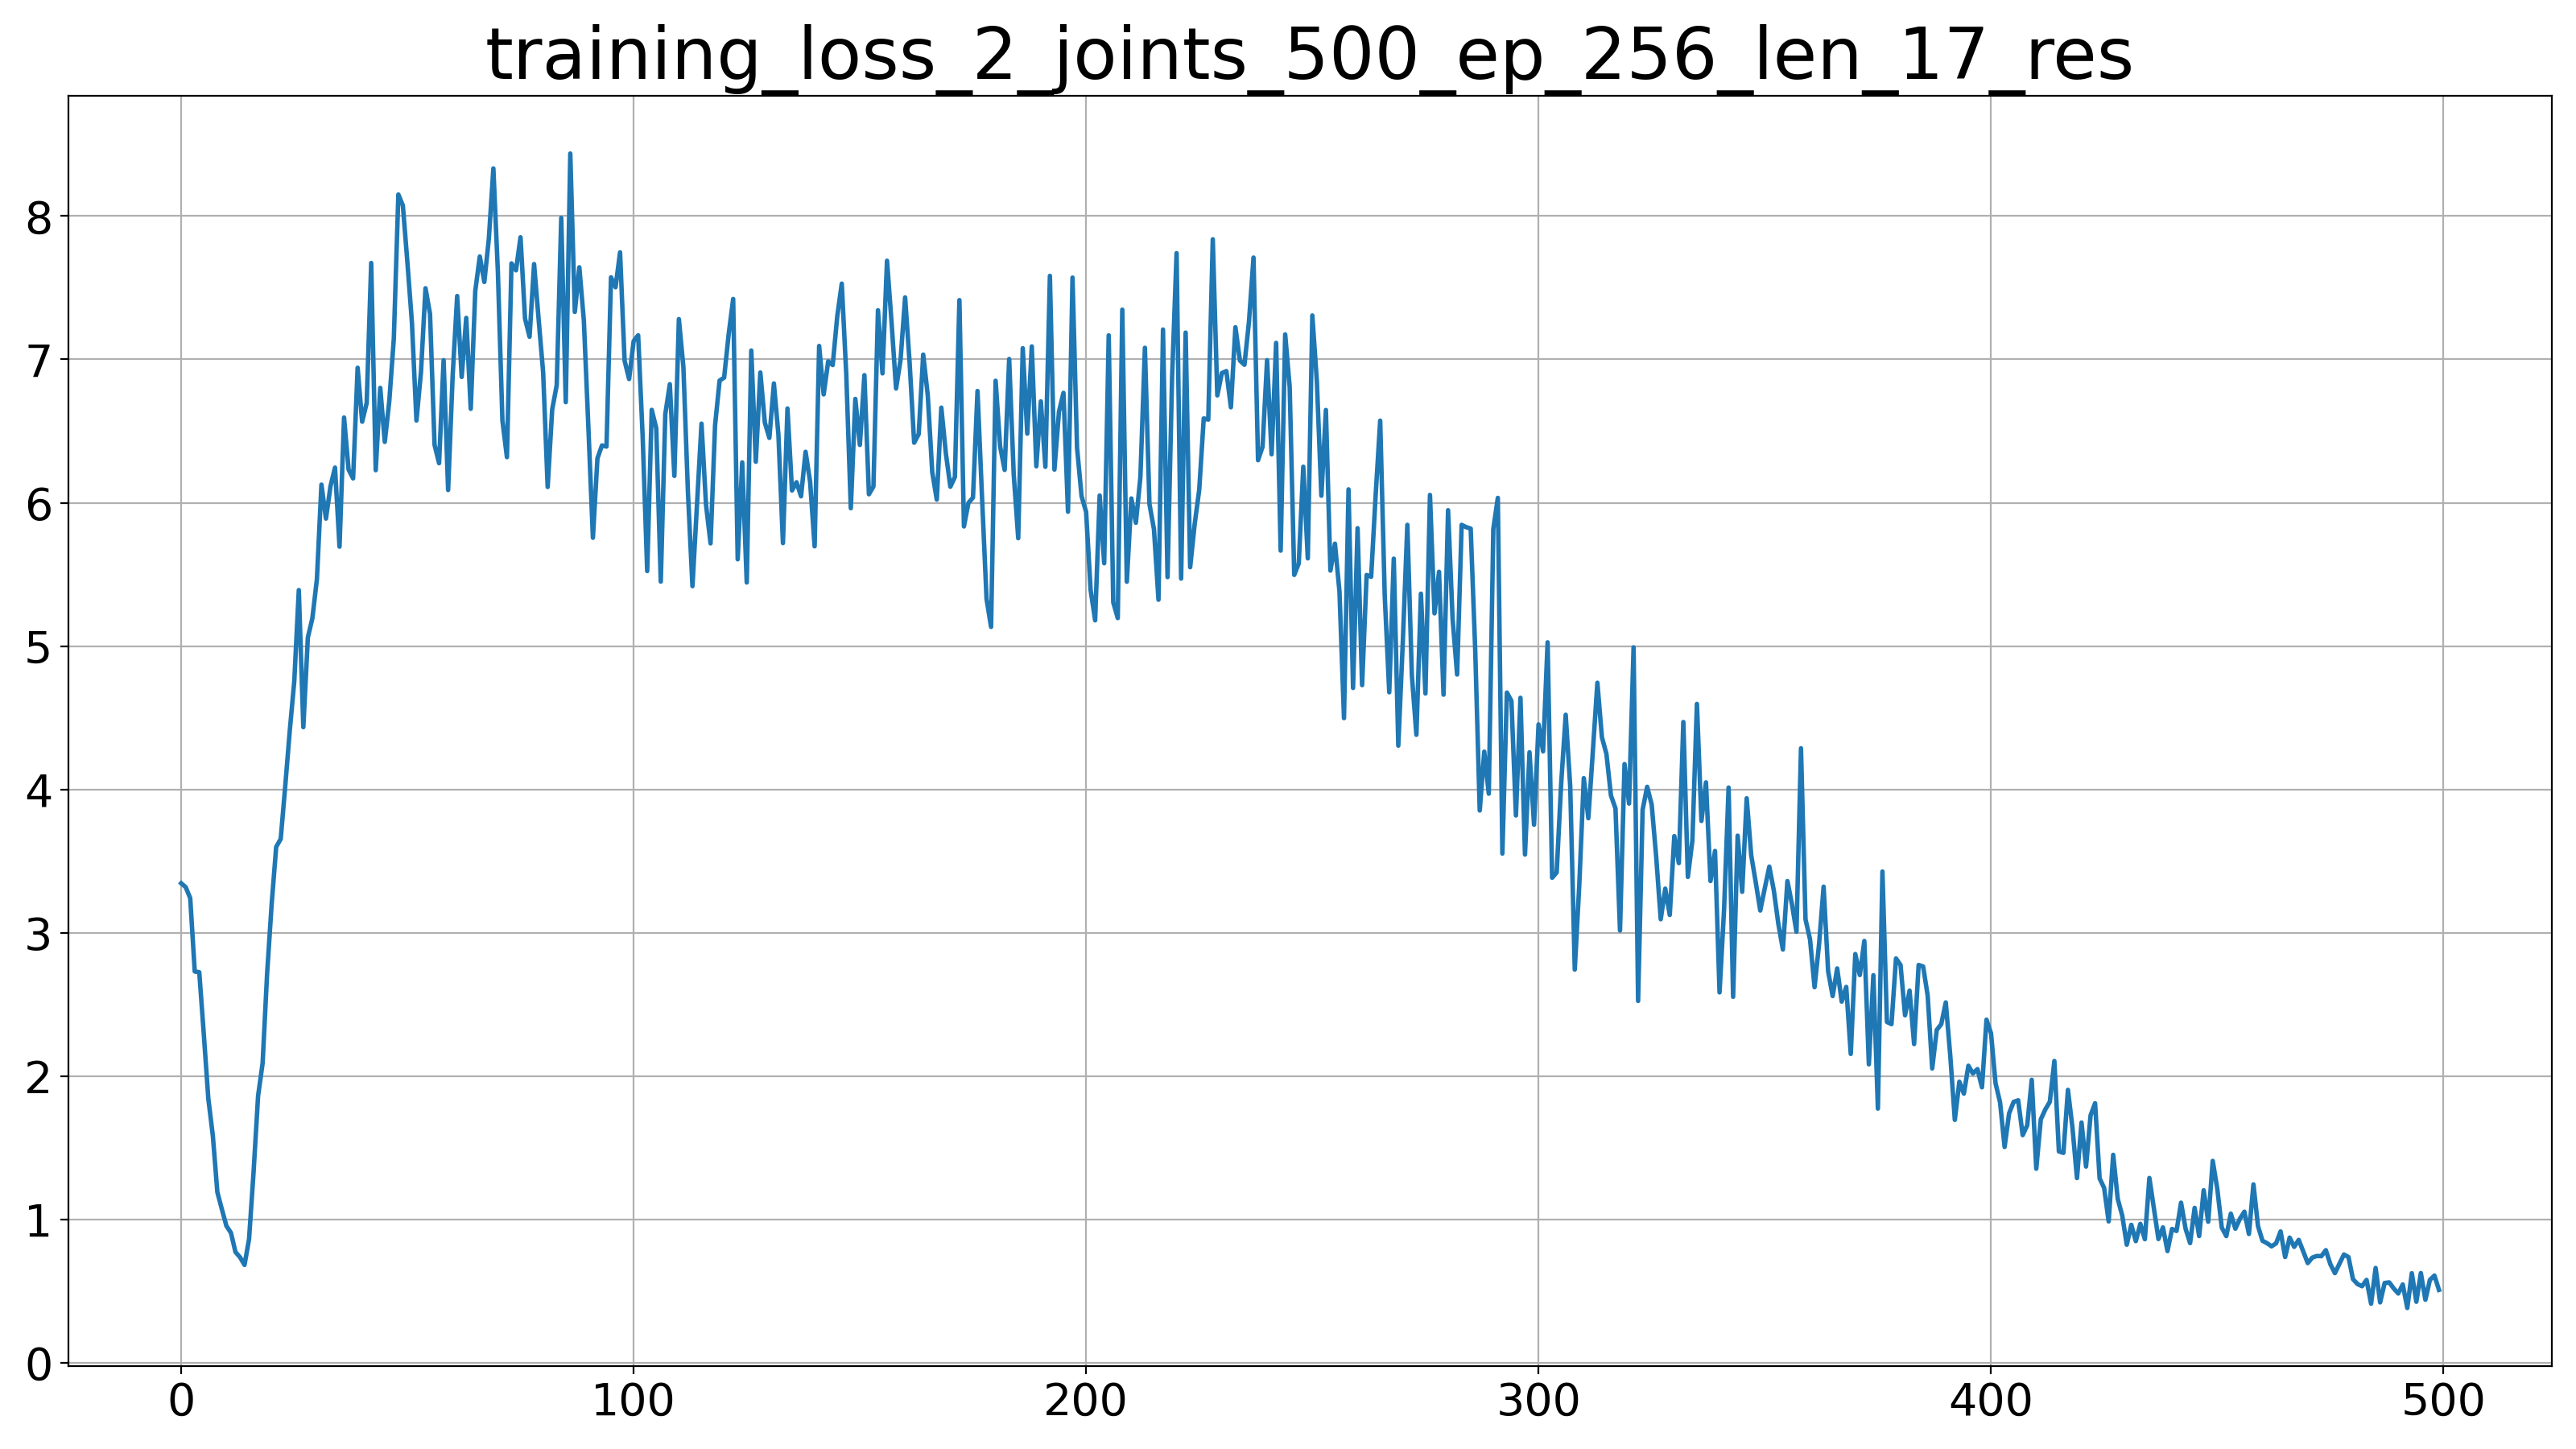
\includegraphics[width=8.5cm]{"../Figures/training_loss_2J_500E_256EL_17RES.png"}
	\caption{Training loss over 500 episodes lasted 256 iterations having 2
			 joint and 17 resolution steps.}
	\label{fig:TrainLoss_2_500_17}
\end{figure}
\vspace{-1cm}

\begin{figure}[H]
	\centering
	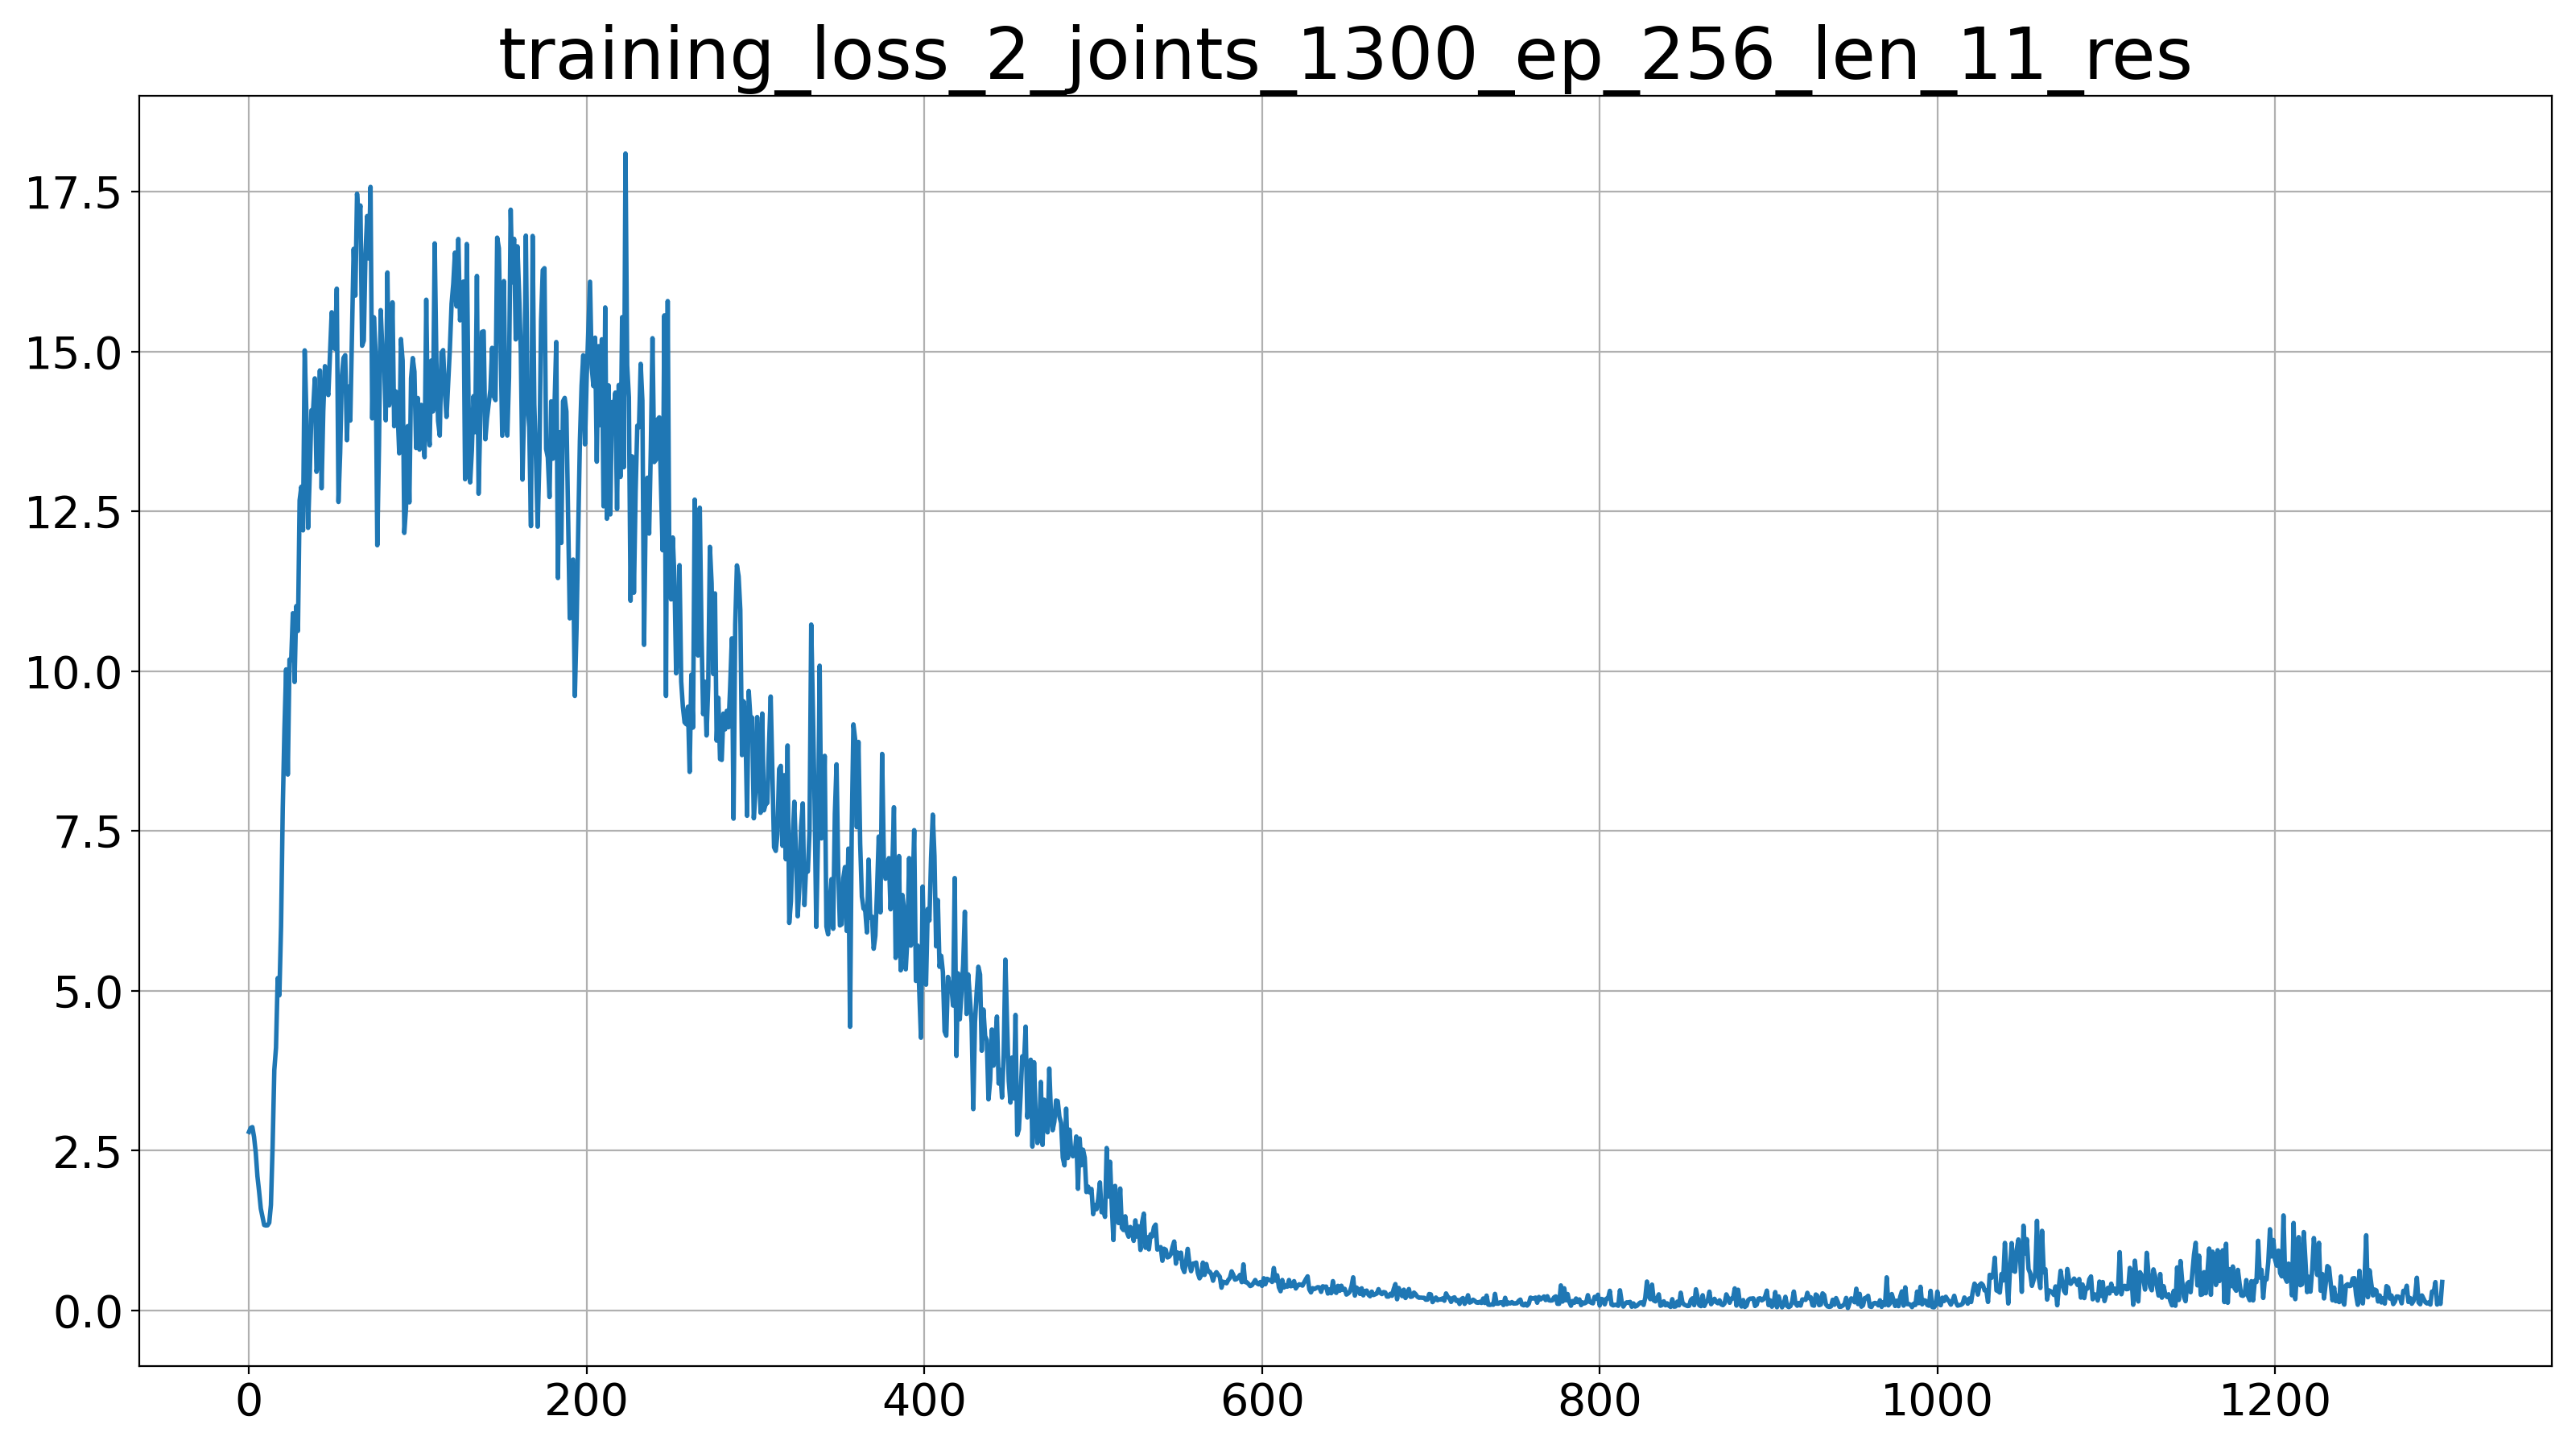
\includegraphics[width=8.5cm]{"../Figures/training_loss_2J_1300E_256EL_11RES.png"}
	\caption{Training loss over 1300 episodes lasted 256 iterations having 2
			 joint and 11 resolution steps.}
	\label{fig:TrainLoss_2_1300_11}
\end{figure}

\begin{figure}[H]
	\centering
	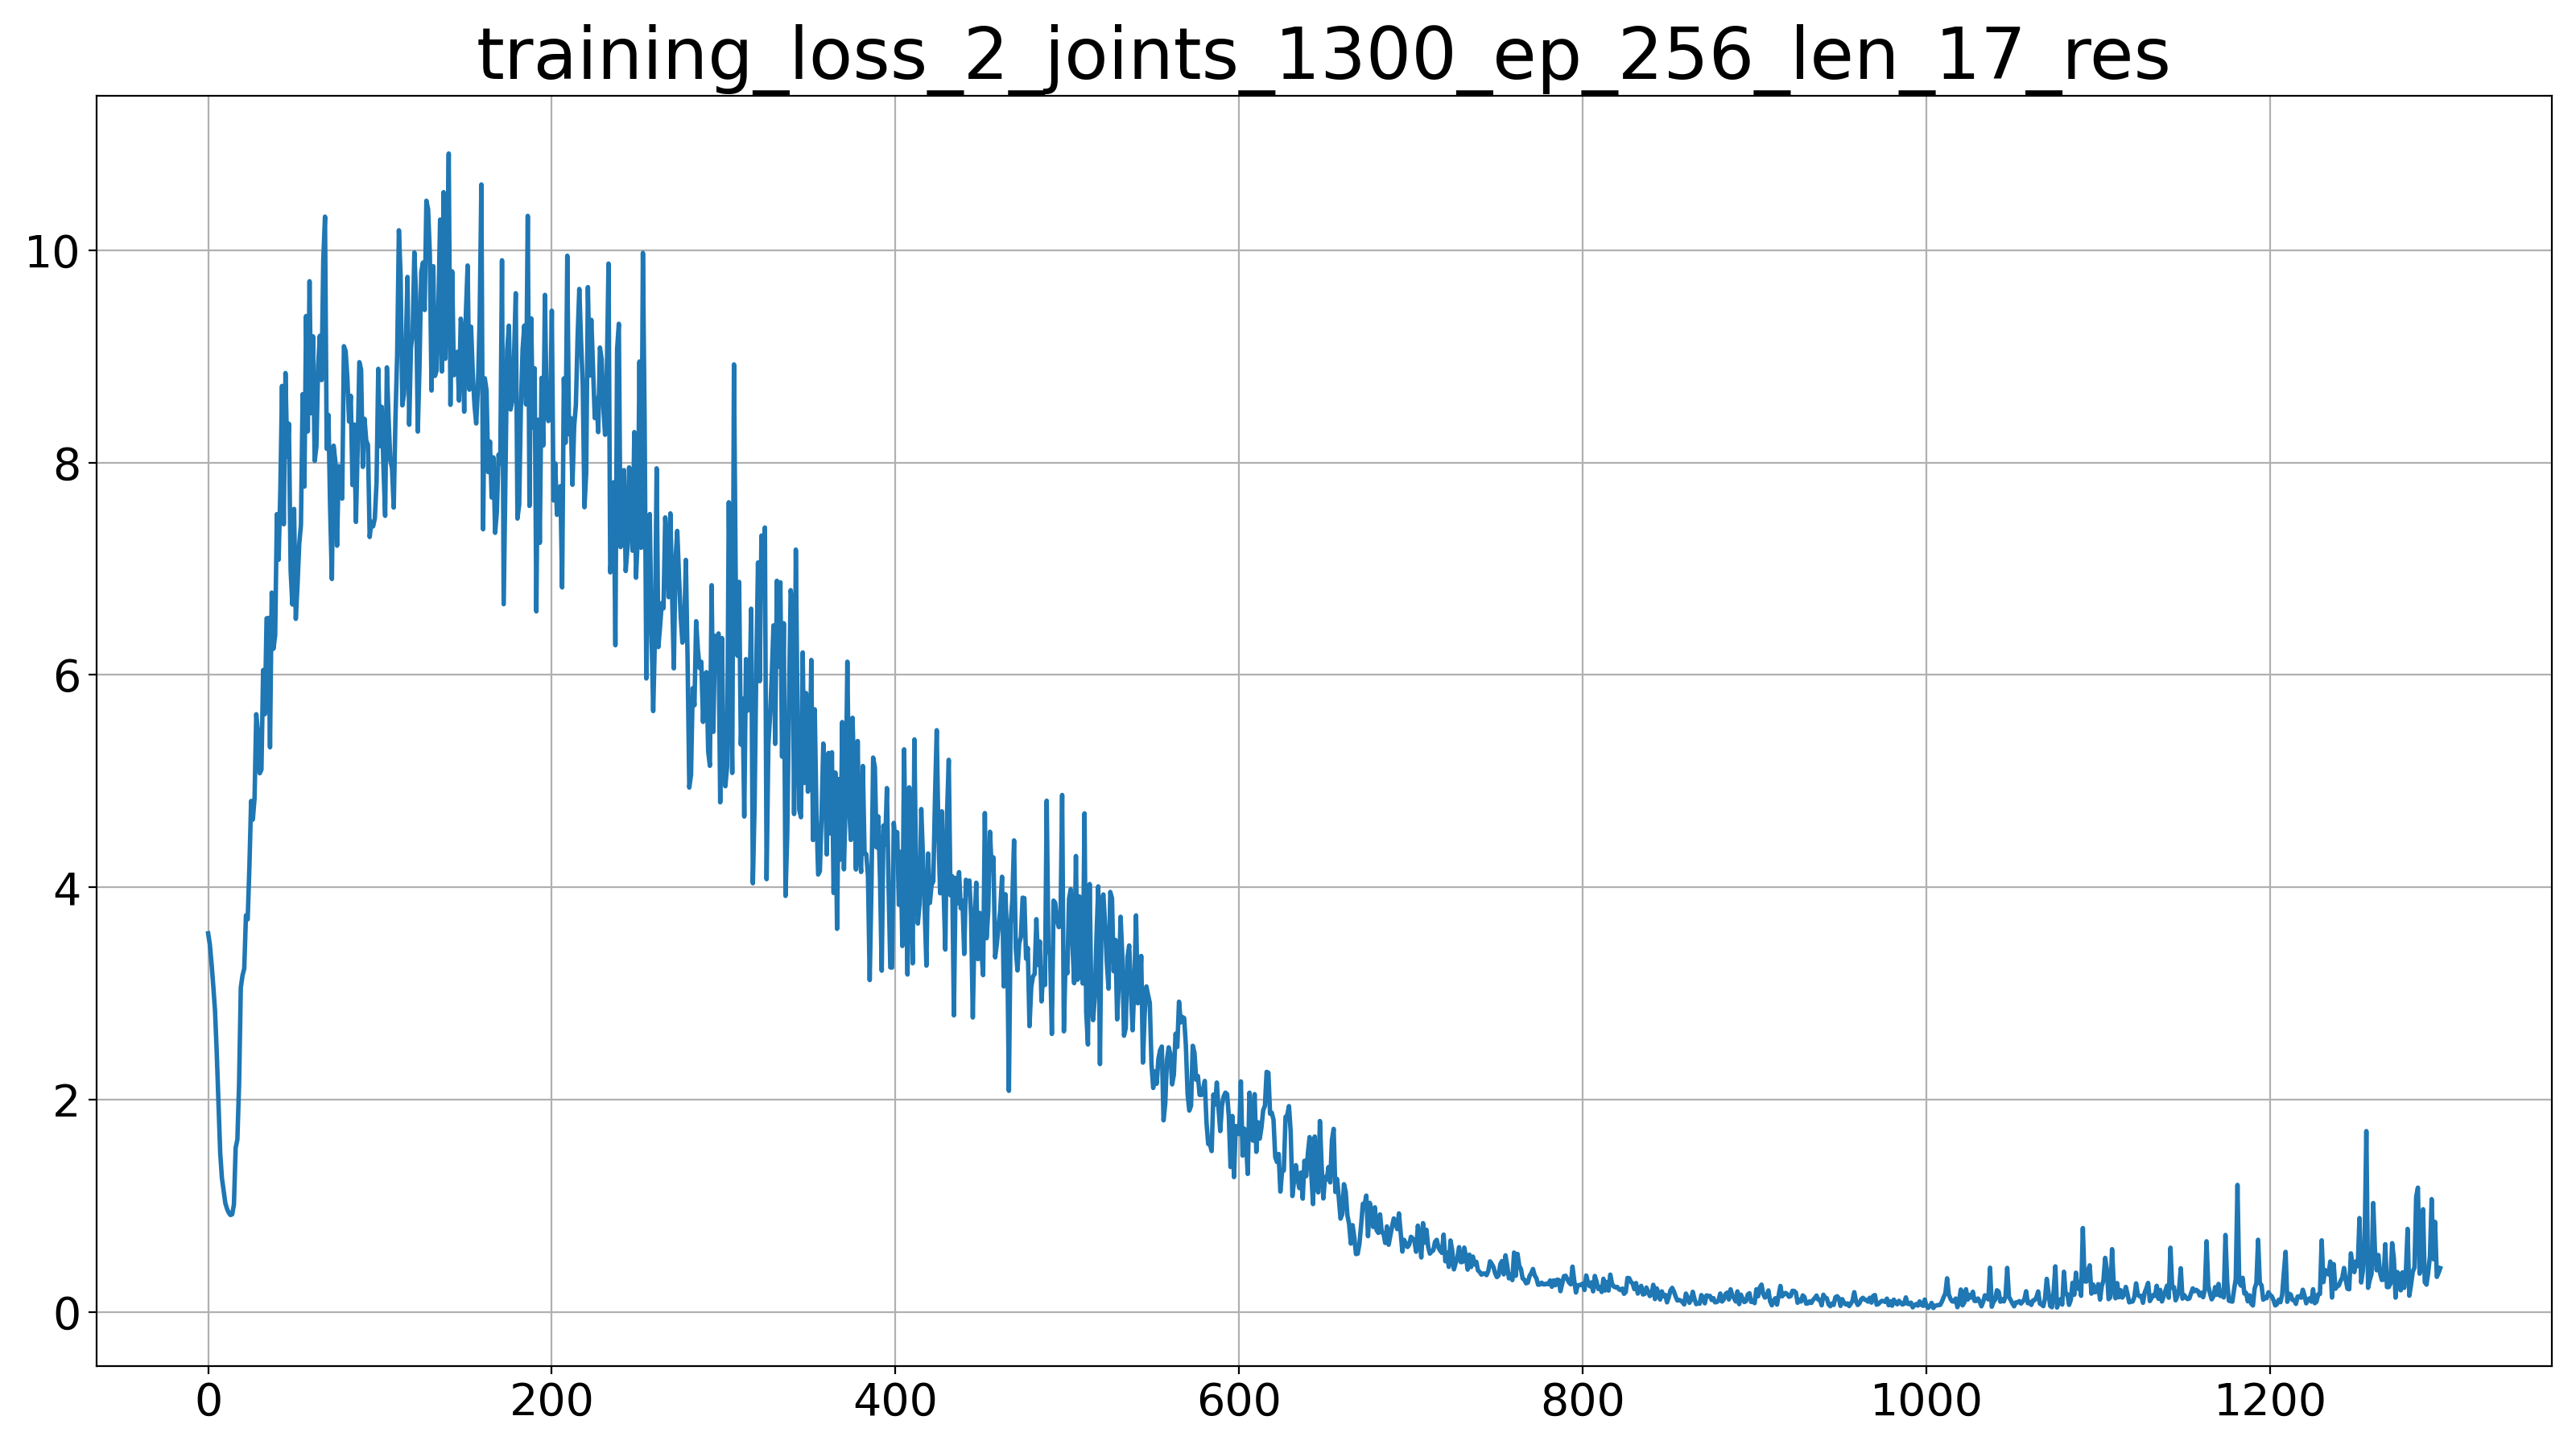
\includegraphics[width=8.5cm]{"../Figures/training_loss_2J_1300E_256EL_17RES.png"}
	\caption{Training loss over 1300 episodes lasted 256 iterations having 2
			 joint and 17 resolution steps.}
	\label{fig:TrainLoss_2_1300_17}
\end{figure}

% Training cost-to-go
Following are the graphs showing the training cost to go, gathered from the
training episodes.

\begin{figure}[H]
	\centering
	\includegraphics[width=8.5cm]{"../Figures/Training_costs_2_joints_500_ep_256_len_11_res.png"}
	\caption{Training cost-to-go over 500 episodes lasted 256 iterations having 2
			 joint and 11 resolution steps.}
	\label{fig:Train_cost_to_go_2_500_11}
\end{figure}

\begin{figure}[H]
	\centering
	\includegraphics[width=8.5cm]{"../Figures/Training_costs_2_joints_500_ep_256_len_17_res.png"}
	\caption{Training cost-to-go over 500 episodes lasted 256 iterations having 2
			 joint and 17 resolution steps.}
	\label{fig:Train_cost_to_go_2_500_17}
\end{figure}

\begin{figure}[H]
	\centering
	\includegraphics[width=8.5cm]{"../Figures/Training_costs_2_joints_1300_ep_256_len_11_res.png"}
	\caption{Training cost-to-go over 1300 episodes lasted 256 iterations having 2
			 joint and 11 resolution steps.}
	\label{fig:Train_cost_to_go_2_1300_11}
\end{figure}
\vspace{-1cm}

\begin{figure}[H]
	\centering
	\includegraphics[width=8.5cm]{"../Figures/Training_costs_2_joints_1300_ep_256_len_17_res.png"}
	\caption{Training cost-to-go over 1300 episodes lasted 256 iterations having 2
			 joint and 17 resolution steps.}
	\label{fig:Train_cost_to_go_2_1300_17}
\end{figure}

Differently from what said in the case of the 1 joint configuration,
the 2 joints one presents strong peaks in the graphs of the training cost to go
explained by the divergence of the network visible in the loss graphs 
represented in Figures \ref{fig:TrainLoss_2_1300_11}.
% Test phase

\begin{figure}[H]
	\centering
	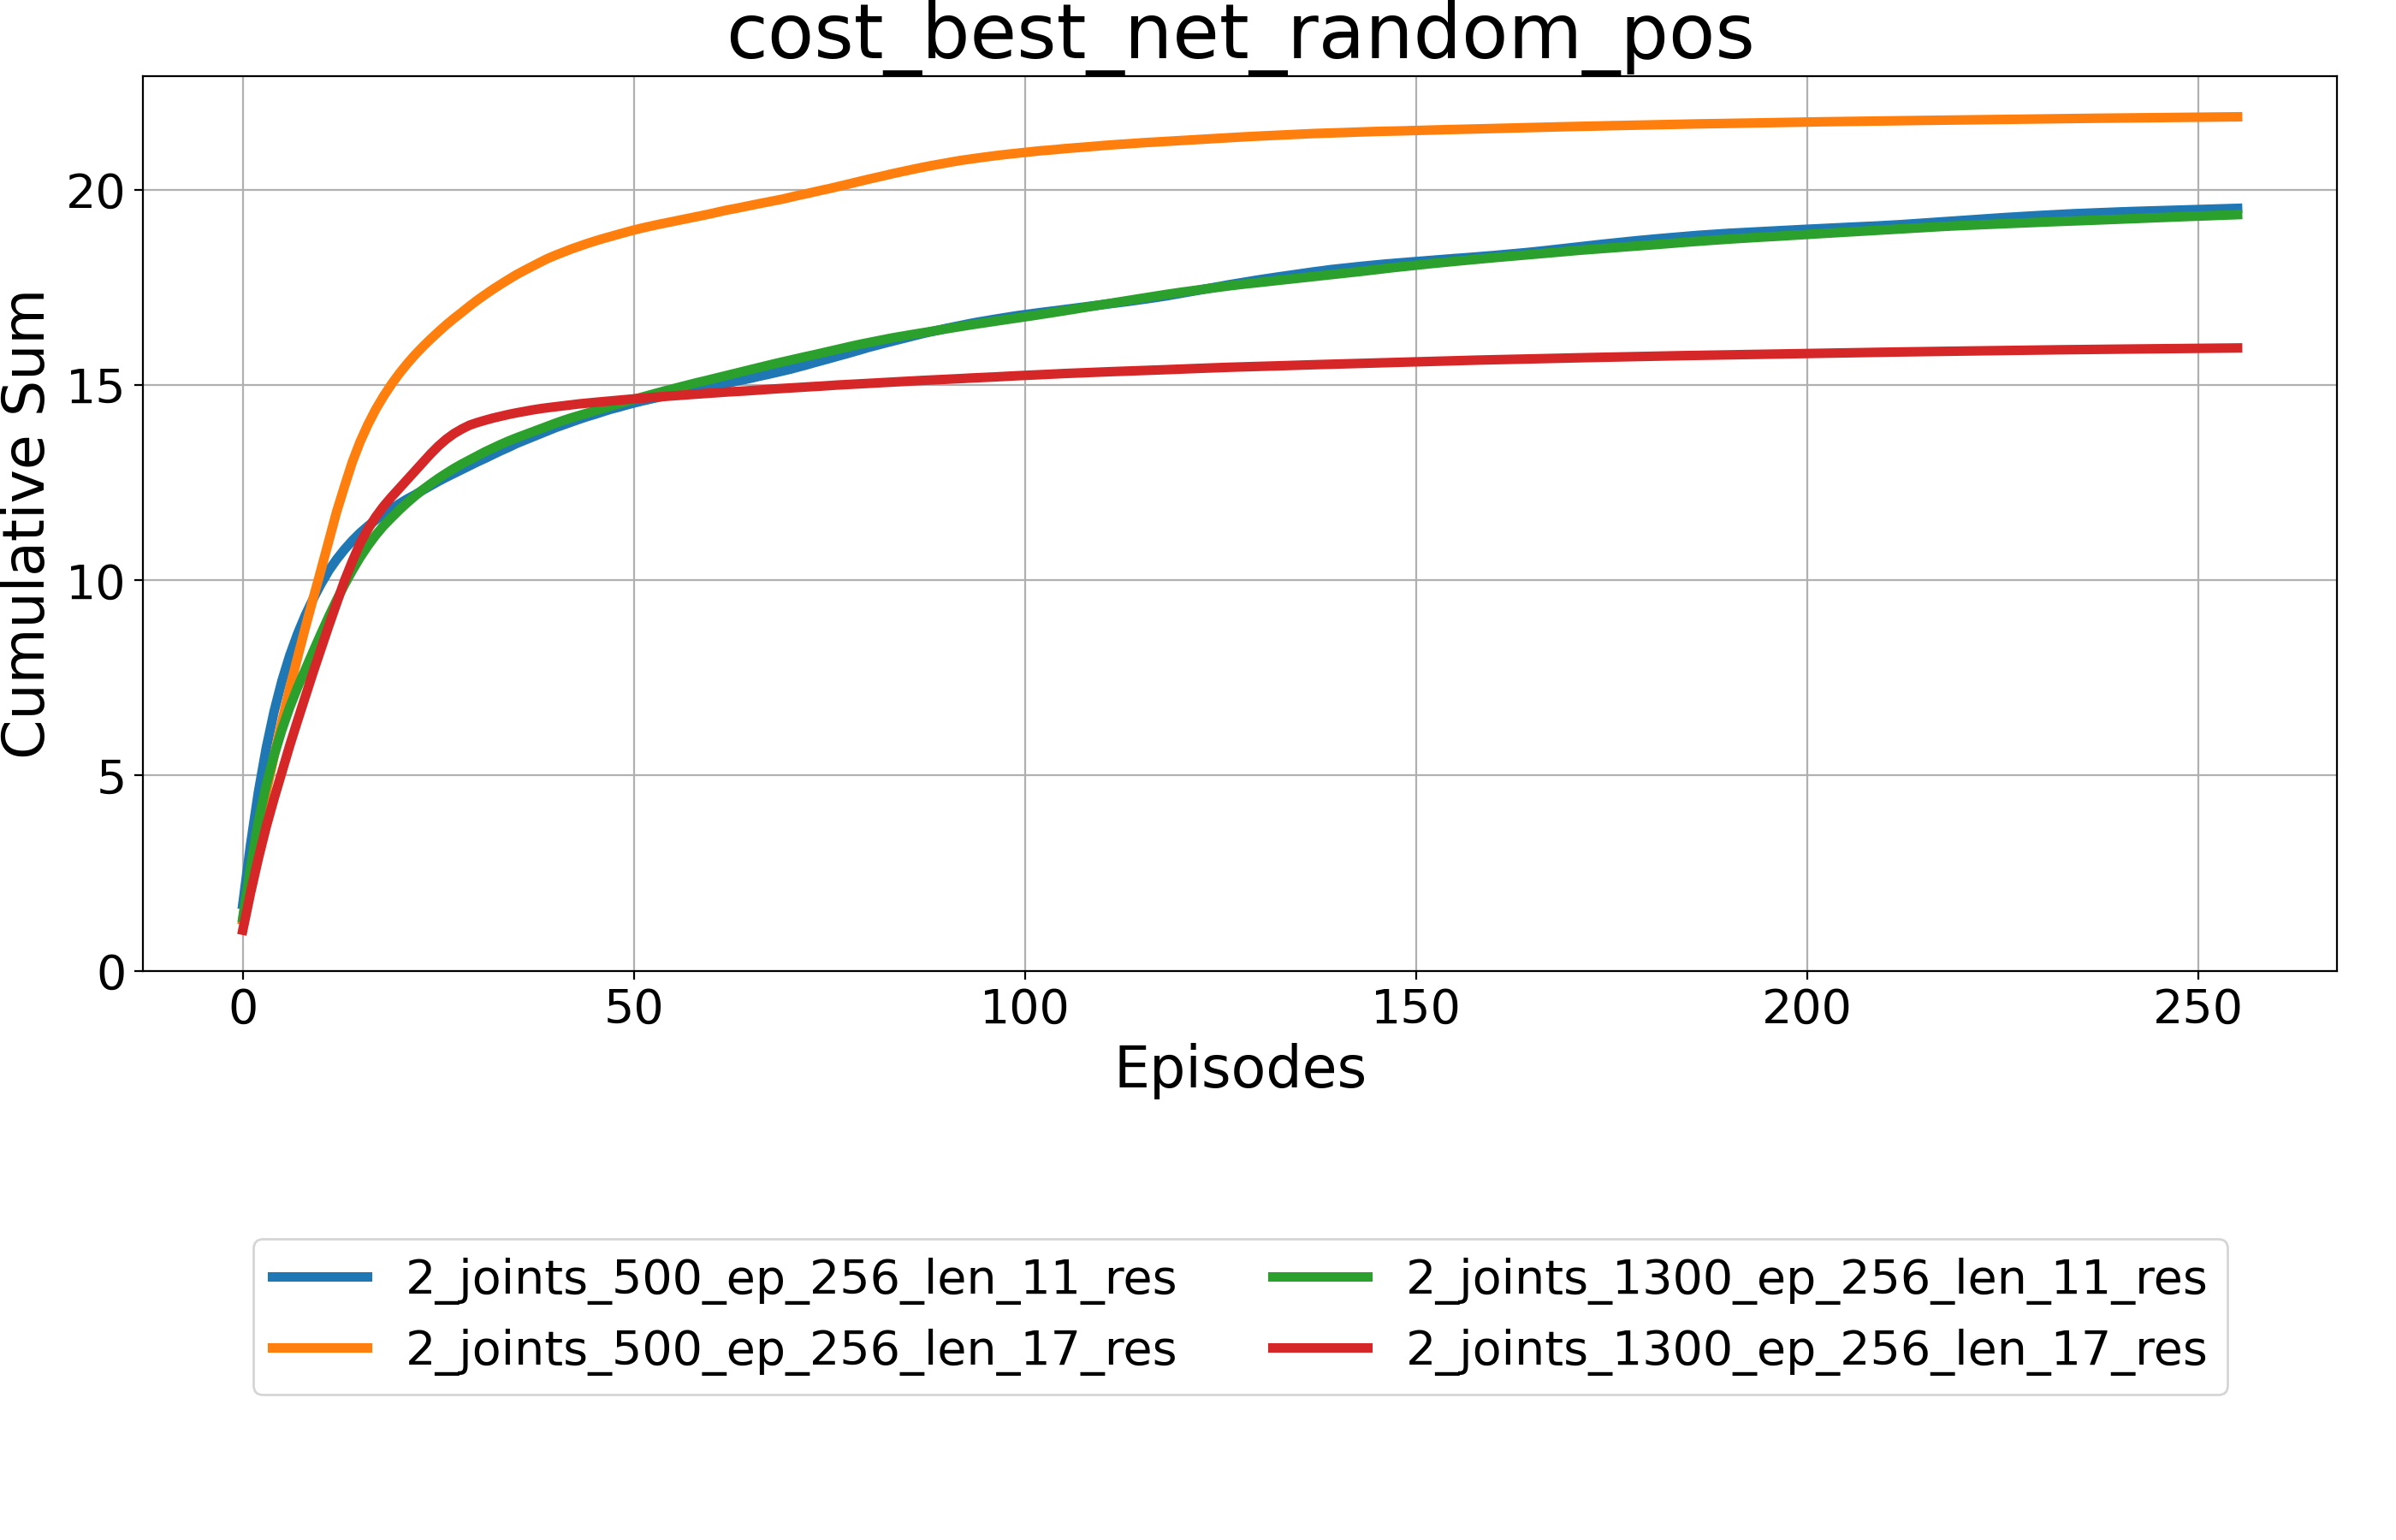
\includegraphics[width=8.5cm]{"../Figures/Summary_cost_best_net_random_pos_2J.png"}
	\caption{Total cost over the test episodes for the robot starting from
			 random positions using the best performing network.}
	\label{fig:Test_2_best_net_random_pos}
\end{figure}
\vspace{-1cm}
\begin{figure}[H]
	\centering
	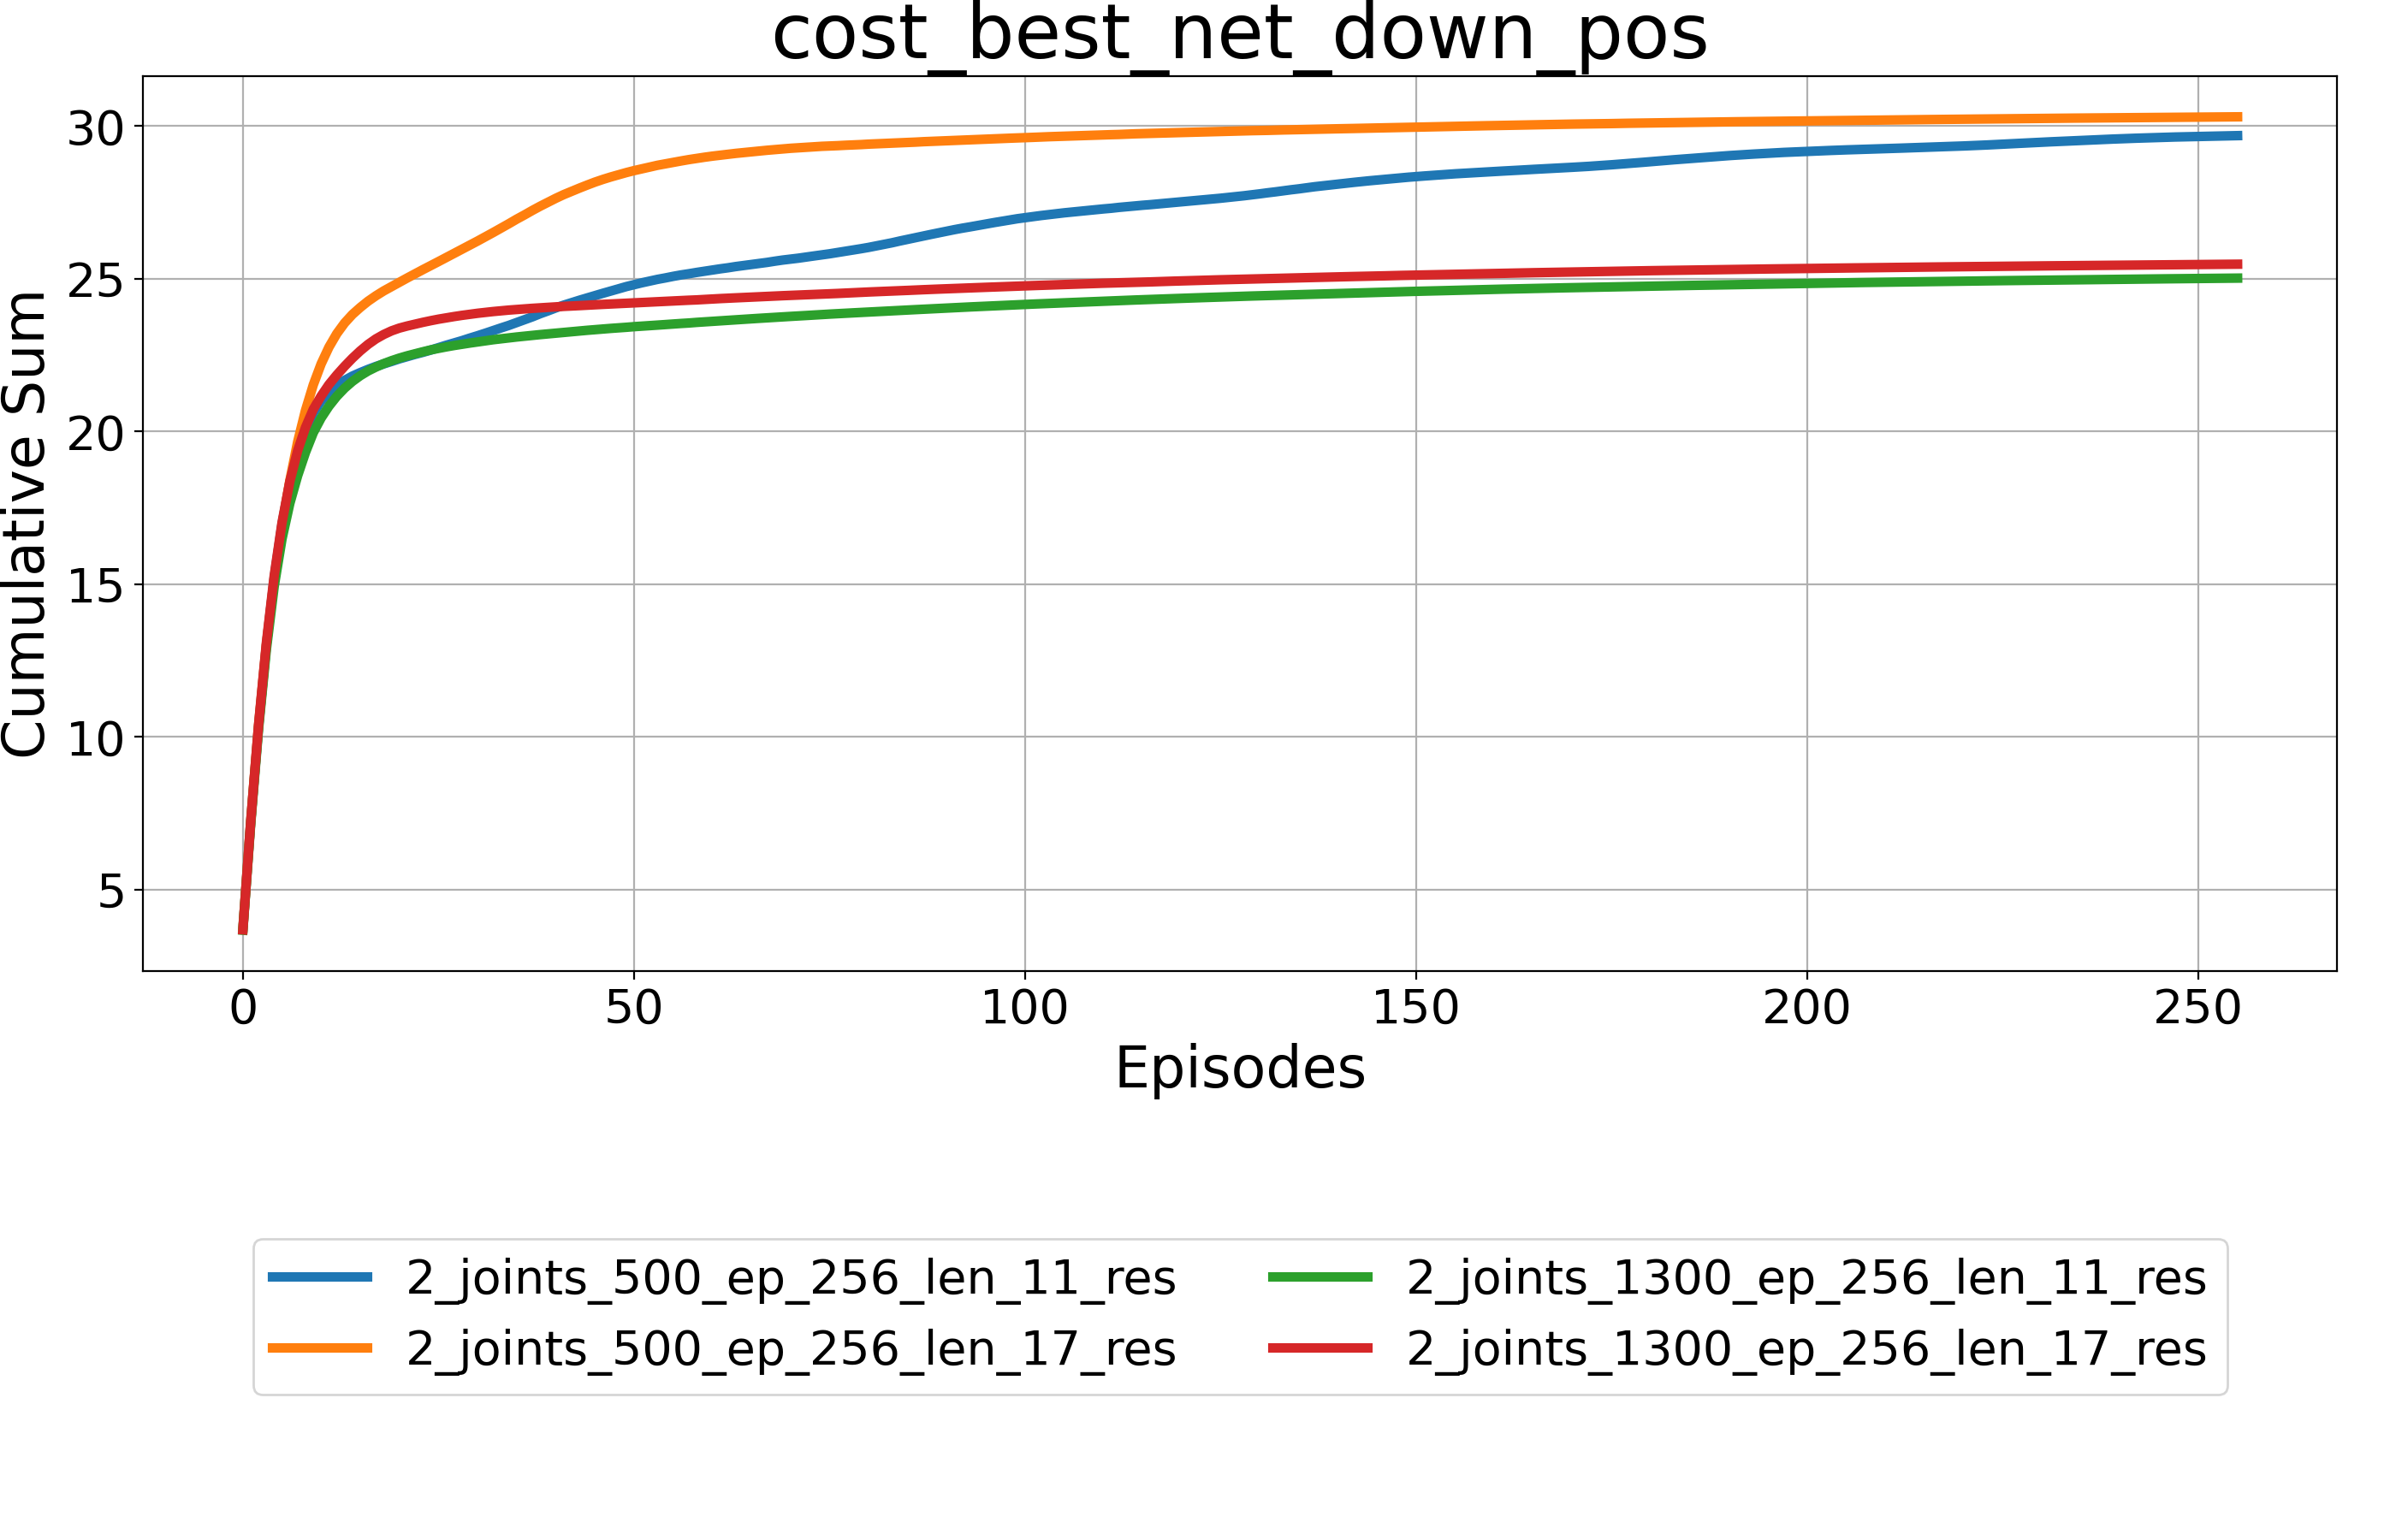
\includegraphics[width=8.5cm]{"../Figures/Summary_cost_best_net_down_pos_2J.png"}
	\caption{Total cost over the test episodes for the robot starting from
			 down positions using the best performing network.}
	\label{fig:Test_2_best_net_down_pos}
	\end{figure}
It is possible to observe how differently from the 1 joint case, the 2 joints
implementation shows a training loss which decreases at around 800 episodes
to then increase again. This behaviour may be due to the non-linear
approximation which does not grant convergence.
Furthermore, in the testing phase, the setting having 1300 episodes and 11
control resolution steps was the one leading to the lowest cumulative cost
as shown in Figures \ref{fig:Test_2_last_ep_random_pos}, \ref{fig:Test_2_last_ep_down_pos} and
\ref{fig:Test_2_best_net_down_pos}, while in Figure \ref{fig:Test_2_best_net_random_pos}
shows the setting 1300 episodes and 17 control resolution steps as the winning one.
\newpage

\section{Conclusion}

\begin{thebibliography}{9}
	\bibitem{Mnih}
	Mnih, V., Kavukcuoglu, K., Silver, D. et al. Human-level control through
	deep reinforcement learning. Nature 518, 529–533 (2015).
	https://doi.org/10.1038/nature14236
	\bibitem{Roderick}
	Roderick M., MacGlashan J., Tellex S. Implementing the Deep Q-Network.
	\href{https://doi.org/10.48550/arXiv.1711.07478}
		 {https://doi.org/10.48550/arXiv.1711.07478}
\end{thebibliography}

\end{document}
